%!TEX root = ../Main.tex

\chapter{System Arkitektur}
\RevisionsTabel{System Arkitektur}{
Alle	& 1.0	& 25-08-15 & Domain \\
Alle 	& 2.0	& 09-10-15 & Dokumentstruktur \\
}

%I system arkitekturen er designet af systemet beskrevet og dokumenteret. Alle aspekter af designet er beskrevet heri, som skal give læseren det fulde indblik i designet af 'navnet på systemmet'\fxnote{Skriv navnet på systemmet her}.

%Dokumentstruktur - valg af N+1 moddellen 
\section{Introduktion}
Projektet er skabt for at tilfredstille de nye behov, som \textit{Katrines Kælder} har ønsket gennem en henvendelse til gruppen. \textit{Katrines Kælder} har ønsket et elektronisk kassesystem, som kan føre journal over det salg, som har været i løbet af en åbningsdag. Kassesystemet skal ligeledes kunnne integrere betalinger fra \textit{Dankort}-terminalen.

\subsection{Formål og omfang}
Formålet med dokumentet er at beskrive arkitekturen bag systemet. Arkitekturen er bygget ud fra de krav, som er stillet i kravspecifikationen. Dokumentet vil beskrive designet af systemet uden at gå i dybden i forhold til implementeringen.

\subsection{Referencer}
Referencer vil kunne findes bagerst i dokumentet i afsnittet.

\subsection{Dokumentstruktur og læsevejledning}
Dokumentstrukturen er bygget op omkring N\plus1 modellen, som er en udvidelse af 4\plus1 modellen. Modellen skaber en beskrivelse af systemet ud fra forskellige synspunkter. Dvs. at de forskellige views behandler arkitekturbeskrivelsen anderledes alt efter hvilket view, der er i fokus. Modsat 4\plus1 modellen, som kan ses i figur~\ref{fig:4plus1}, kan N\plus1 indeholde alle de views, som der nødvendige for at skrive en komplet dokumentation af systemet.

\begin{figure}[H]
	\centering
	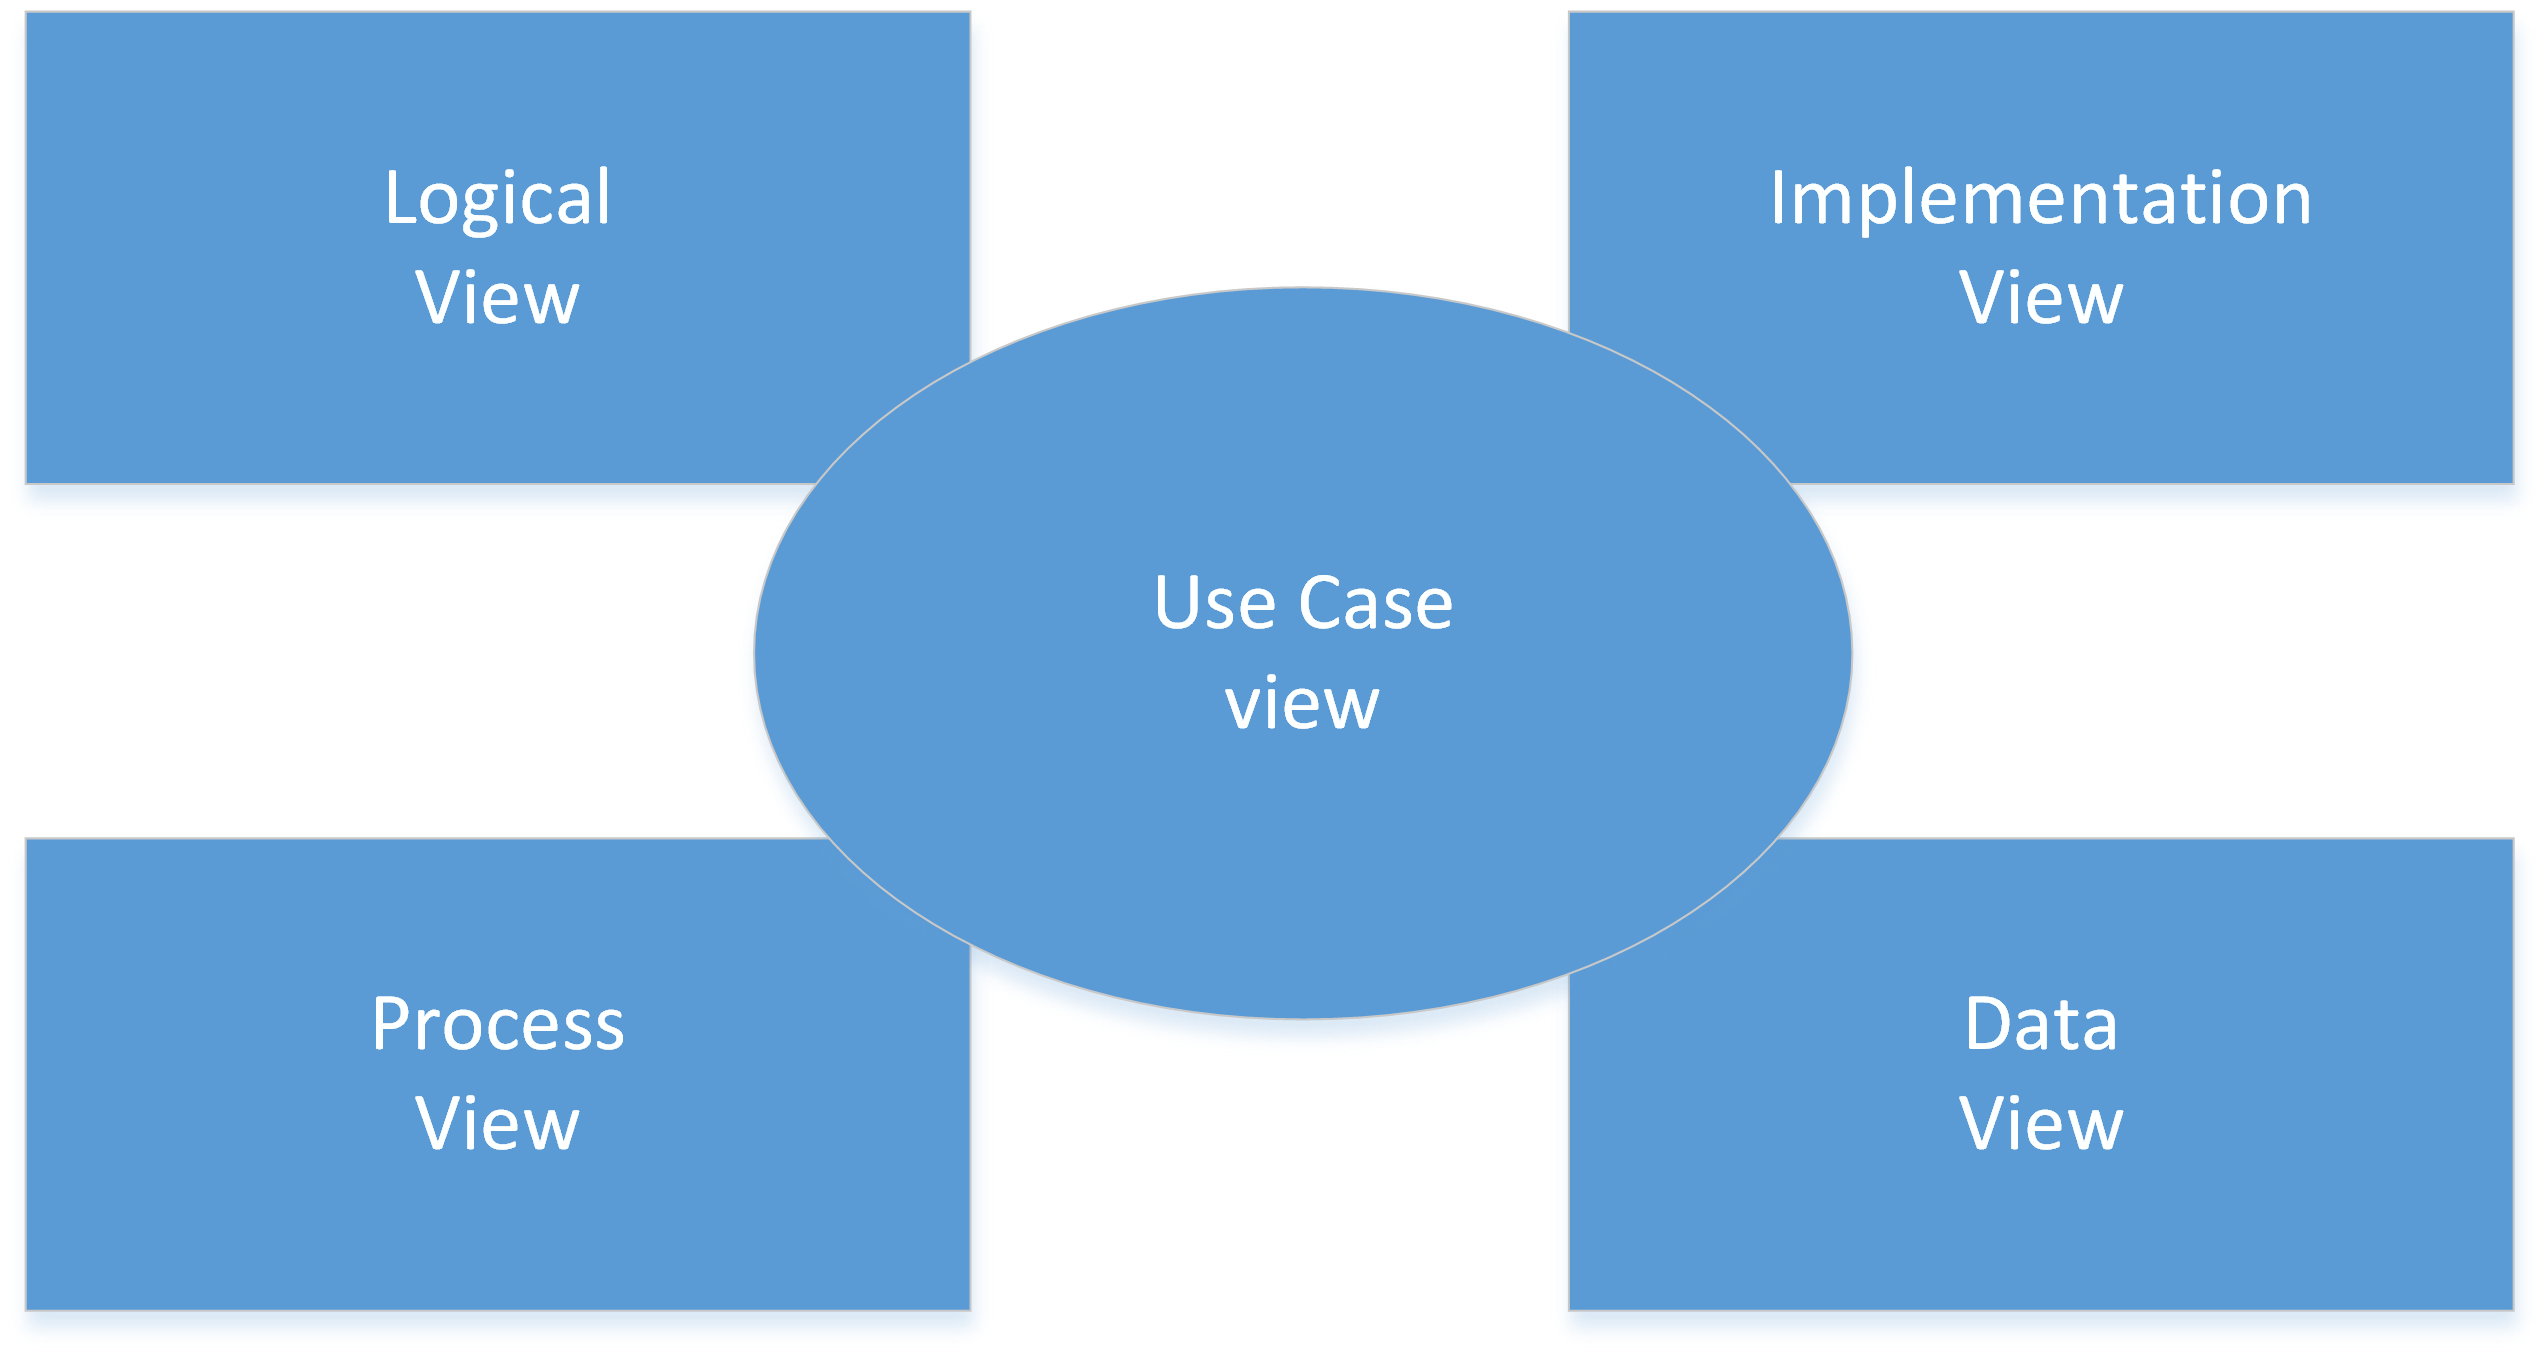
\includegraphics[width=0.7\textwidth]{N+1/Intro/Nplus1.png}
	\caption{4 plus 1 modellen}
	\label{fig:4plus1}
\end{figure}

I dette dokument har vi valgt at indkludere følgende views:

\begin{itemize}
	\item Domain View
	\item Use Case View
	\item Logical View
	\item Process View
	\item Implementation View
	\item Data View
\end{itemize}

\subsubsection{Læsevejledning}
Dokumentet læses fortløbende for at opnå en fuld forståelse af systemet. Enkelte afsnit har referencer tilbage til kravspecifikationen, der skal ses som fundamentet for arkitekturdokumentationen.

\subsection{Dokumentets rolle i en iterativ udviklingsproces}
Dokumentet er en opsamling på det iterative projektarbejde. 
Det er tænkt at dokumentet opdateres løbende med nye use cases og nye realiseringer af disse. 
Det gør at dokumentet virker som en vejledning hvorfra systemet kan implementeres. 
Når der arbejdes iterativt giver det rigtigt god mening at have et dokument der fastsætter hvilke aftaler der er lavet for nuværende sprint.

%System oversigt
\section{System oversigt}
Dette afsnit skal give et overblik over systemets hensigt og omgivelser. Da meget af den informationen allerede findes i kravspecifikationen, kan dette afsnittet ses, som en kort opsamling af de informationer.

\subsection{System kontekst}
Ud fra henvendelsen fra \textit{Katrines Kælder} er der blevet tegnet et aktør-kontekst diagram. Diagrammet kan findes i kravspecifikationen i afsnit~\ref{sec:actors}, som figur~\ref{fig:actordiagram}. Her findes også beskrivelser af systemets aktører.

\subsection{System introduktion}
Målet med projektet er at implementere et system, som kan føre journal. Dette indbærer at registrere salg af et produkt og samle det i en ordre. Ordrene skal persisteres i en database, som kan gøre en behandling af dataene muligt. Dette kunne f.eks. være i forhold til at lave en kasseafstemning, hvor dagens salg skal udregnes og sammenlignes med den totale omsætning. Transaktioner opbevares også med de forskellige ordre.
\newline\newline
Et af målene er også at integrere \text{Dankort}-transaktioner i systemet. Her skulle det være muligt at opstille en transaktion samt fra systemets side at godtage transaktionen.

%System grænseflade
\section{Systemets grænseflader}
Dette afsnit vil beskrive systemet grænseflader.

\subsection{Grænseflader til person aktører}
Systemet har to person grænseflader: Bartender og Admin.
\newline\newline
Bartender kan vha. brugergrænsefladen:
\begin{itemize}
	\item Udføre salg
	\item Tage imod betaling
\end{itemize}

Admin kan vha. WebAPI'et:
\begin{itemize}
	\item Oprette, redigere og slette produkter.
\end{itemize}

\subsection{Grænseflader til eksterne system aktører}
Systemet har tre eksterne system aktører: Nets, MobilePay og Swipp. Nets -- altså Dankort -- har været første prioritet i forhold til betalingsudbydere. Da systemet stadig i udviklingsfasen, hvor Dankort skal implementeres vil Nets kun blive beskrevet i dette afsnit.
\newline\newline
Nets er udbyderen af Dankort systemet. Systemet skal interagere med den API, som er stillet til rådighed fra Nets. Selve API'en og interaktionen med systemet er ikke undersøgt nærmere. 

%\subsection{Grænseflader til hardware aktører}

%\subsection{Grænseflader til eksterne software aktører}

%Use Case View
\section{Use Case View}
De forskellige usecase kan ses under Kravspecifikationen.

% Sekvensdiagrammer
%!TEX root = ../../main.tex

\subsection{OverordnedeSekvensDiagrammer}
I dette afsnit vises de overordnede sekvensdiagrammer som er lavet med det formål at kunne vise interaktionen mellem aktør og systemet. Samtidig viser der også systemets funktionalitet i henhold til kravspecifikationen, og derfor at gøre det lettere at forstå systemet i forhold til den ydre verden. 


\subsubsection{Overordnet sekvensdiagram for Use Case 1 ''Kontant salg''}
Diagrammet viser interaktion mellem Bartender og system for Use Case 1, ''Kontant Salg'' 

\sysml{0.6}{SEQ}{UseCase1}{Use Case 1}

Som der kan ses på på sekvensdiagrammet figur \ref{fig:UseCase1_SEQ}, har bartenderen mulighed for at opdaterer betalings listen inde i et loop, indtil alle bestillingerne er tastet ind. For at komme ud af loopet skal Bartenderen enten annullerer købet eller gå til Betaling. 


\subsubsection{Overordnet sekvensdiagram for Use Case 2 ''Udskriv kundebon''}
Diagrammet viser interaktion mellem Bartender og system for Use Case 2, ''Kontant Salg'' 

\sysml{0.6}{SEQ}{UseCase2}{Use Case 2}

Når Bartender printer en Bon kan skal systemmet udskrive en bon, men i tilfælde af at der ikke er mere papir vil systemmet melde en besked om at der ikke er mere papir.
\newline\newline
For at se hvordan man skifter Bon papiret skal man se under Use Case 2 - Extension 2.1.



\subsubsection{Overordnet sekvensdiagram for Use Case 3 ''Kasseafstemning''}
Diagrammet viser interaktion mellem Bartender og system for Use Case 3, ''Kasseafstemning'' 

\sysml{0.6}{SEQ}{UseCase3}{Use Case 3}

Når Bartender skal afstemme kassen afslutter han Use Casen med udskiver en udskrive en bon over afstemningen, men i tilfælde af at der ikke er mere papir vil systemmet melde en besked om at der ikke er mere papir.
\newline\newline
For at se hvordan man skifter Bon papiret skal man se under Use Case 3 - Extension 3.2.


\subsubsection{OverOrdnet sekvensdiagram for Use Case 9 ''Tilføj varer til kasseapparat''}
Diagrammet viser interaktionen mellem Admin system for Use Case 9, ''Tilføj varer til kasseapparat''.

\sysml{1.0}{SEQ}{UseCase9}{Use Case 9}

Når Admin skal tilføje en vare starter han Web API'et op og indskriver varen dér. Når han er færdig vil varen kunne vises på Systemet GUI. 

\subsubsection{Overordnet sekvensdiagram for Use Case 10 ''Rediger varer i kasseapparat''}
Diagrammet viser interaktionen mellem Admin og system for Use Case 10, ''Rediger varer i kasseapparat''.

\sysml{1.0}{SEQ}{UseCase10}{Use Case 10}

Når Admin skal redigere et produkt starter han Web API'et op og vælger det produkt han vil ændrer. Når han er færdig, kan det opdaterede produkt ses på systemets GUI.

\subsubsection{Overordnet sekvensdiagram for Use Case 11 ''Fjern varer fra kasseapparat''}
Diagrammet viser interaktionen mellem Admin og system for Use Case 11, ''Fjern varer i kasseapparat''.

\sysml{1.0}{SEQ}{UseCase11}{Use Case 11}

Når Admin skal fjerne et produkt, starter han Web API'et op og vælger det produkt der ønskes fjernet. Når han er færdig, vil det fjernede produkt ikke vises på systemets GUI.

\subsubsection{Overordnet sekvensdiagram for Use Case 12 ''Vis statistik over salg''}
Diagrammet viser interaktionen mellem Admin og system for Use Case 12 ''Vis statistik over salg''.

\sysml{1.0}{SEQ}{UseCase12}{Use Case 12}

Når Admin skal se statistik over salg, starter han Web API'et op og vælger siden der viser statistikken over salg.  

%Domain View
\section{Domænemodel}
Ud fra de definerede use-cases i kravspecifikationen er følgende klasser og interfaces blevet udledt. Klassediagrammet i figur~\ref{fig:CashRegister_DOMAIN} tager udgangspunkt i \texttt{ICashRegister}. Denne har forbindelse til \texttt{GUI}, som er en \textit{boundry} klasse dvs. en klasse, som er udefrakommendes vej til brug af systemet. Klassen \texttt{CashRegister} skal varetage systemets funktionalitet såsom opsætning af salg, gennemførelse af transaktion, udprintning af bon osv.

\sysml{0.9}{DOMAIN}{CashRegister}{ICashRegister}

I figur~\ref{fig:PaymentMethodController_DOMAIN} klassen. Denne skal håndtere hvilke betalingsmetoder, som skal bruges under en transaktion. Klassen har forbindelse til \texttt{IPrint}, som skal printe en bon og \texttt{IDrawer}, der skal kunne åbne skuffen.

\sysml{0.5}{DOMAIN}{PaymentMethodController}{IPaymentMethodController}
%http://www.tutorialspoint.com/design_pattern/data_access_object_pattern.htm
I figur~\ref{fig:ProductController_DOMAIN} ses klassen \texttt{ProductController}. Klassen står for håndteringen af \texttt{Product}'s (varer) i systemet. Klassen skal kunne tilføje, slette og ændre i systemets varekartotek. Disse ændringer skal derefter videreformidles til databasen gennem \texttt{IProductDao} -- en såkaldt \textit{Dao} (Data Access Object Pattern) implementation. Implementeringen \texttt{ProductDaoImpl} omsætter systemet \texttt{Product}'s til database information, som derefter kan skubbes ind i databasen gennem interfacet \texttt{IDatabase}.

\sysml{0.6}{DOMAIN}{ProductController}{IProductController}

I figur~\ref{fig:ProductGroupController_DOMAIN} ses klassen \texttt{ProductGroupController}. Klassen står for behandle de forskellige \texttt{Product}'s i deres respektive \texttt{ProductGroup}'s (varegrupper). Denne bruger ligeledes \textit{Dao} implementationen til kommunikationen mellem systemet og databasen.

\sysml{0.6}{DOMAIN}{ProductGroupController}{IProductGroupController}

I figur~\ref{fig:DiscountController_DOMAIN} ses klassen \texttt{DiscountController}. Klassen skal holde styr på de rabat, som kan gives på varerne. Der gøres heri ligeledes brug af \textit{Dao}.

\sysml{0.6}{DOMAIN}{DiscountController}{IDiscountController} 

I figur~\ref{fig:ReceiptController_DOMAIN} ses klassen \texttt{ReceiptController}. Klassen skal opbevare de salg, som er foretaget i løbet af en salgsdag. Salgene bliver skrevet ind i databasen, hvilket kan tages ud igen, når der skal dannes en dagssalgs kvittering.

\sysml{0.6}{DOMAIN}{ReceiptController}{IReceiptController}

I figur~\ref{fig:Log_DOMAIN} ses klasserne \texttt{Log}, \texttt{Printer} og \texttt{FilePrinter}. \texttt{Log} står for at logge hændelser i programmet, som har værdi. Hændelserne bliver sendt videre til et interface \texttt{IPrinter} hovedsageligt klassen \texttt{FilePrinter}, som udskriver til en bestemt fil, hvor alle de loggede hændelser står. Klassen \texttt{Printer} er en implementering til bonprinteren, der skal udskrive bon, dagssalg osv.

\sysml{0.6}{DOMAIN}{Log}{ILog og IPrinter}

Det fleste af systemets klasser har kendskab til \texttt{ILog}. Dette er dog ikke tegnet på diagrammerne. Hændelser gennem klassehierakiet kan derved logges.

%Logical View
\section{Logical View}
Dette kapitel beskriver systemets opdeling i delsystemer. Her ser vi på de funktionaliteter som systemmet giver til brugeren. 

\subsection{Oversigt}
\logicalview{0.80}{PKG}{System}{System}

For at gøre systemet overskuelig har vi inddelt systemet i flere lag. Således at vi adskiller \Gls{brugergraenseflade} og \Gls{forretningslogik} samt \gls{DAL}. I figur \ref{fig:System_PKG} kan det ses at hver af de store pakker er inddelt i flere små pakker som hver har deres eget ansvar hvilket vil blive beskrevet i følgende afsnit.

\subsection{Arkitektursignifikante designpakker	}
\subsubsection{Pakke 1: GUI}

\subsubsection{Pakke 2: Business Layer}
I dette afsnit beskrives koden i projektets business layer
\subsection{Sales}
%\section{Logical View}
Dette kapitel beskriver systemets opdeling i delsystemer. Her ser vi på de funktionaliteter som systemmet giver til brugeren. 

\subsection{Oversigt}

\subsection{Arkitektursignifikante designpakker	}
\subsubsection{Pakke 1: GUI}


\subsubsection{Pakke 2: Business Layer}
%\input{Systemarkitektur/LogicalView/BusinessLayer}


\subsubsection{Pakke 3: Data}

\subsection{Use Case realiseringer	}
\subsubsection{ Use Case 1. realisering	}
\subsubsection{ Use Case 2. realisering	}



\subsection{Orders}
%\input{Systemarkitektur/LogicalView/BusinessLayer/Order}

\subsection{Payment}
%\section{Logical View}
Dette kapitel beskriver systemets opdeling i delsystemer. Her ser vi på de funktionaliteter som systemmet giver til brugeren. 

\subsection{Oversigt}

\subsection{Arkitektursignifikante designpakker	}
\subsubsection{Pakke 1: GUI}


\subsubsection{Pakke 2: Business Layer}
%\input{Systemarkitektur/LogicalView/BusinessLayer}


\subsubsection{Pakke 3: Data}

\subsection{Use Case realiseringer	}
\subsubsection{ Use Case 1. realisering	}
\subsubsection{ Use Case 2. realisering	}



\subsection{Products}
%\input{Systemarkitektur/LogicalView/BusinessLayer/Product}

\subsection{CashDrawers}
%\section{Logical View}
Dette kapitel beskriver systemets opdeling i delsystemer. Her ser vi på de funktionaliteter som systemmet giver til brugeren. 

\subsection{Oversigt}

\subsection{Arkitektursignifikante designpakker	}
\subsubsection{Pakke 1: GUI}


\subsubsection{Pakke 2: Business Layer}
%\input{Systemarkitektur/LogicalView/BusinessLayer}


\subsubsection{Pakke 3: Data}

\subsection{Use Case realiseringer	}
\subsubsection{ Use Case 1. realisering	}
\subsubsection{ Use Case 2. realisering	}



\subsection{Receipts}
%\section{Logical View}
Dette kapitel beskriver systemets opdeling i delsystemer. Her ser vi på de funktionaliteter som systemmet giver til brugeren. 

\subsection{Oversigt}

\subsection{Arkitektursignifikante designpakker	}
\subsubsection{Pakke 1: GUI}


\subsubsection{Pakke 2: Business Layer}
%\input{Systemarkitektur/LogicalView/BusinessLayer}


\subsubsection{Pakke 3: Data}

\subsection{Use Case realiseringer	}
\subsubsection{ Use Case 1. realisering	}
\subsubsection{ Use Case 2. realisering	}



\subsection{Printer}
%\textbf{Printer pakken}
\newline
Printer pakken er lavet for at gøre det muligt for programmet at udskrive kvitteringer samt at udskrive afstemningen af kassen.
Til dette er der lavet et interface \texttt{IPrinter}. \texttt{IPrinter} er lavet for at gøre det nemt at udskifte printer implementationen.
Interfacet er lavet til at modtage en linje ad gangen.
Selve klassen \texttt{ReceiptPrinter} er lavet til at kunne printe via Windows Printer Dialogen til standard printeren.

\logicalview{0.55}{CLASS}{Printer}{pakken Printer}


\subsection{Models}
%\section{Logical View}
Dette kapitel beskriver systemets opdeling i delsystemer. Her ser vi på de funktionaliteter som systemmet giver til brugeren. 

\subsection{Oversigt}

\subsection{Arkitektursignifikante designpakker	}
\subsubsection{Pakke 1: GUI}


\subsubsection{Pakke 2: Business Layer}
%\input{Systemarkitektur/LogicalView/BusinessLayer}


\subsubsection{Pakke 3: Data}

\subsection{Use Case realiseringer	}
\subsubsection{ Use Case 1. realisering	}
\subsubsection{ Use Case 2. realisering	}



\subsection{Log}
%\section{Logical View}
Dette kapitel beskriver systemets opdeling i delsystemer. Her ser vi på de funktionaliteter som systemmet giver til brugeren. 

\subsection{Oversigt}

\subsection{Arkitektursignifikante designpakker	}
\subsubsection{Pakke 1: GUI}


\subsubsection{Pakke 2: Business Layer}
%\input{Systemarkitektur/LogicalView/BusinessLayer}


\subsubsection{Pakke 3: Data}

\subsection{Use Case realiseringer	}
\subsubsection{ Use Case 1. realisering	}
\subsubsection{ Use Case 2. realisering	}



\subsection{Database}
%\section{Logical View}
Dette kapitel beskriver systemets opdeling i delsystemer. Her ser vi på de funktionaliteter som systemmet giver til brugeren. 

\subsection{Oversigt}

\subsection{Arkitektursignifikante designpakker	}
\subsubsection{Pakke 1: GUI}


\subsubsection{Pakke 2: Business Layer}
%\input{Systemarkitektur/LogicalView/BusinessLayer}


\subsubsection{Pakke 3: Data}

\subsection{Use Case realiseringer	}
\subsubsection{ Use Case 1. realisering	}
\subsubsection{ Use Case 2. realisering	}



\subsection{Dal}
%\section{Logical View}
Dette kapitel beskriver systemets opdeling i delsystemer. Her ser vi på de funktionaliteter som systemmet giver til brugeren. 

\subsection{Oversigt}

\subsection{Arkitektursignifikante designpakker	}
\subsubsection{Pakke 1: GUI}


\subsubsection{Pakke 2: Business Layer}
%\input{Systemarkitektur/LogicalView/BusinessLayer}


\subsubsection{Pakke 3: Data}

\subsection{Use Case realiseringer	}
\subsubsection{ Use Case 1. realisering	}
\subsubsection{ Use Case 2. realisering	}





\subsubsection{Pakke 3: Data}
Database designet er en to delt affære. Der er selve strukturen i databasen også er der koden som tilgår databasen.
Disse beskrive begge i følgende afsnit.

\subsubsection{Database Opbygning}
Opbygning goes here.

\subsubsection{Database kode}
For at kunne tilgå databasen fra C\# blev det besluttet at bruge \gls{EF}. 

\subsection{Use Case realiseringer	}
\subsubsection{ Use Case 1. realisering	}
\subsubsection{ Use Case 2. realisering	}



%Process View
\section{Process View}


%Implementation View 
\section{Implementation View}


%Data View
\section{Data View}
I dette afsnit bliver der lavet en præsentation af koblingen fra objekter til databasen, for at komme tæt på overgangen fra databasen til Businesslayer\fxnote{glossary} og det generelle design bag databasen. Derefter vil der blive overblik over data flows i forhold til nogle udvalgte use cases, som bliver vist med UML aktivitetsdiagrammer, som er kommenteret med de overvejelser og tanker der er gjort bag dem. 

\subsection{Kobling fra database til objekt}
For at mappe databasen til objekter anvendes property mapping, som simpelt er at tablerne koblet til model klasserne og kolonerne er koblet til attributterne. Via et Data Structure Diagram illustreres den fysiske data model, her kan hele diagrammet ses på figur \ref{fig:DSD}.

\begin{figure}[H]
    \centering
    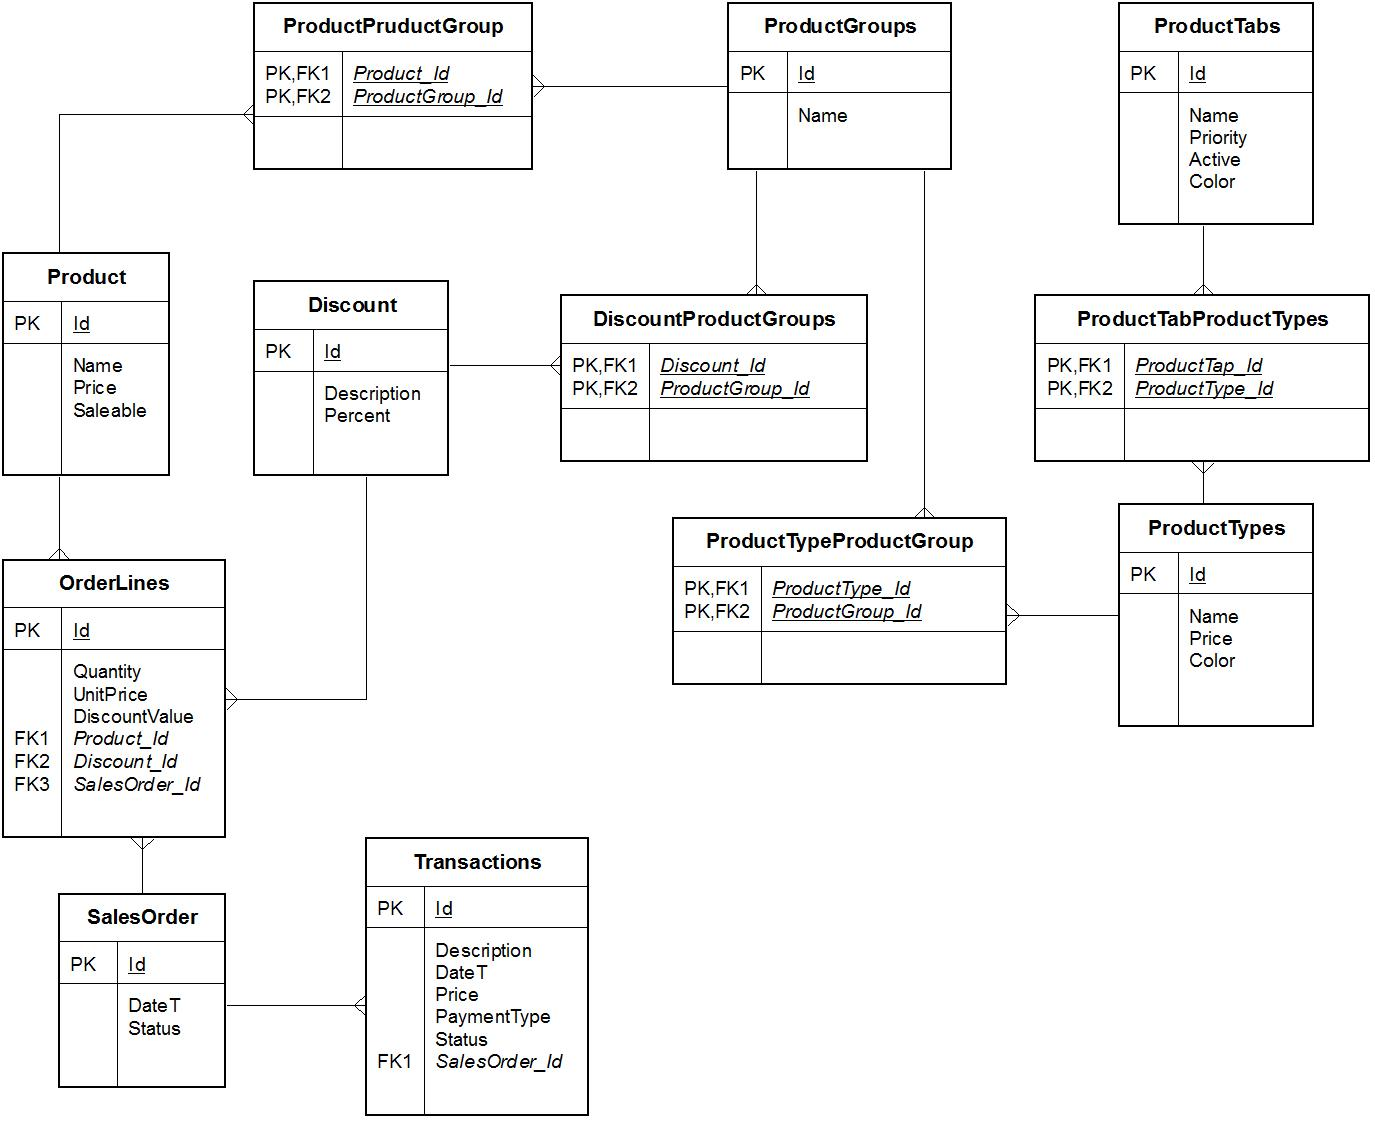
\includegraphics[width=1\textwidth]{N+1/DataView/DabDSD}
    \caption{fysisk data model}
    \label{fig:DSD}
\end{figure}

For at gøre det mere overskueligt vil koblingen af den fysiske data model og klasse modellerne blive delt op i flere diagrammer, hvor der vil være lidt forklaringer på hvorfor databasen er blevet sat om som den er og hvordan det er løst med model klasserne. Her kan hele pakken for model klasserne ses på figur \fxnote{reference til model pakken}.

\subsubsection{Transaction og SalesOrder}
På figur \ref{fig:Mapping_TS} ses koblingen af tabellen Transaction\fxnote{glossery} og SalesOrder\fxnote{glossery} tabellerne

\begin{figure}[H]
    \centering
    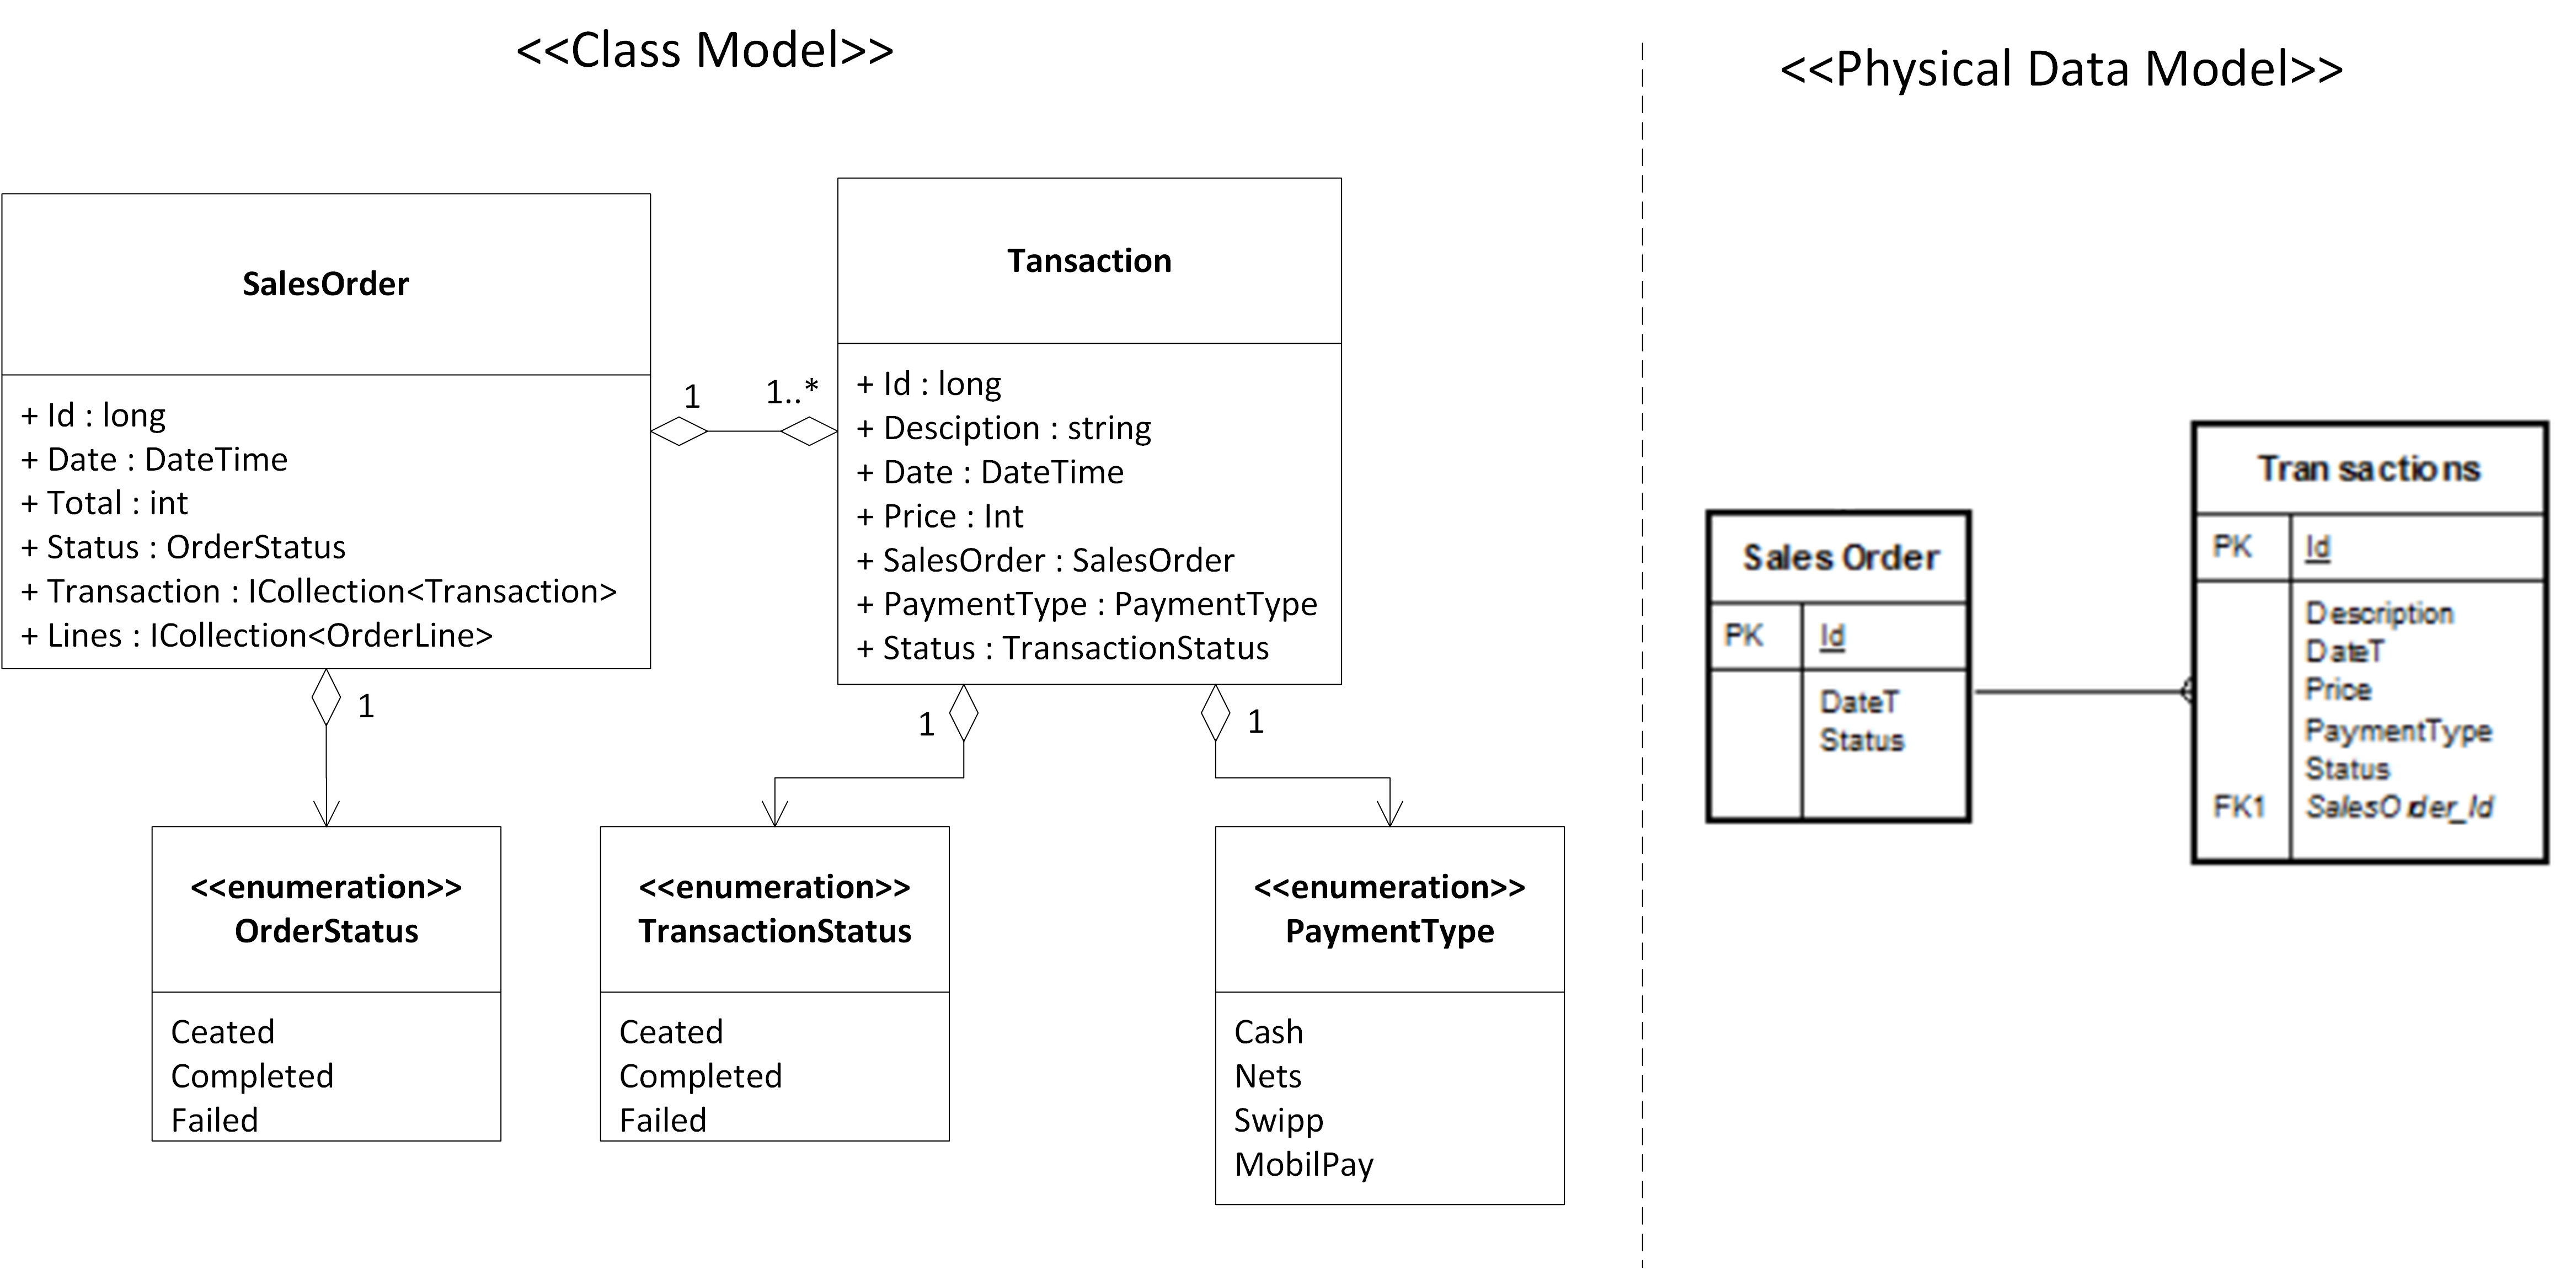
\includegraphics[width=1\textwidth]{N+1/DataView/mapping/Mapping1}
    \caption{kobling af Transaction og SalesOrder}
    \label{fig:Mapping_TS}
\end{figure}

Her kan det ses at attributterne i klasse modellen er minder meget om kolonerne i tabellerne, med nogle få forskelle. En lille ting man kan ligge mærke til er at PaymentType\fxnote{glossery} og Status\fxnote{glossery} er gemt som integer, da navne på dem er gemt i nogle enums inde i C\# koden. 
\newline\newline
Hvis man ser på den fysiske data model, kan det ses at Sales order har en one-to-many forhold, da det skal være muligt for kunden at betale med flere betalingsformer under et salg. For at oversætte denne til klasse modelen har SalesOrder en ICollection af Transactions, så man ud fra sales kan tilgå alle de Transactioner der har været brugt. 

\subsubsection{OrderLine}
På figur \ref{fig:Mapping_Orderline} ses kobling af OrderLine, Product, Discount og SalesOrder\fxnote{glossery}. 

\begin{figure}[H]
    \centering
    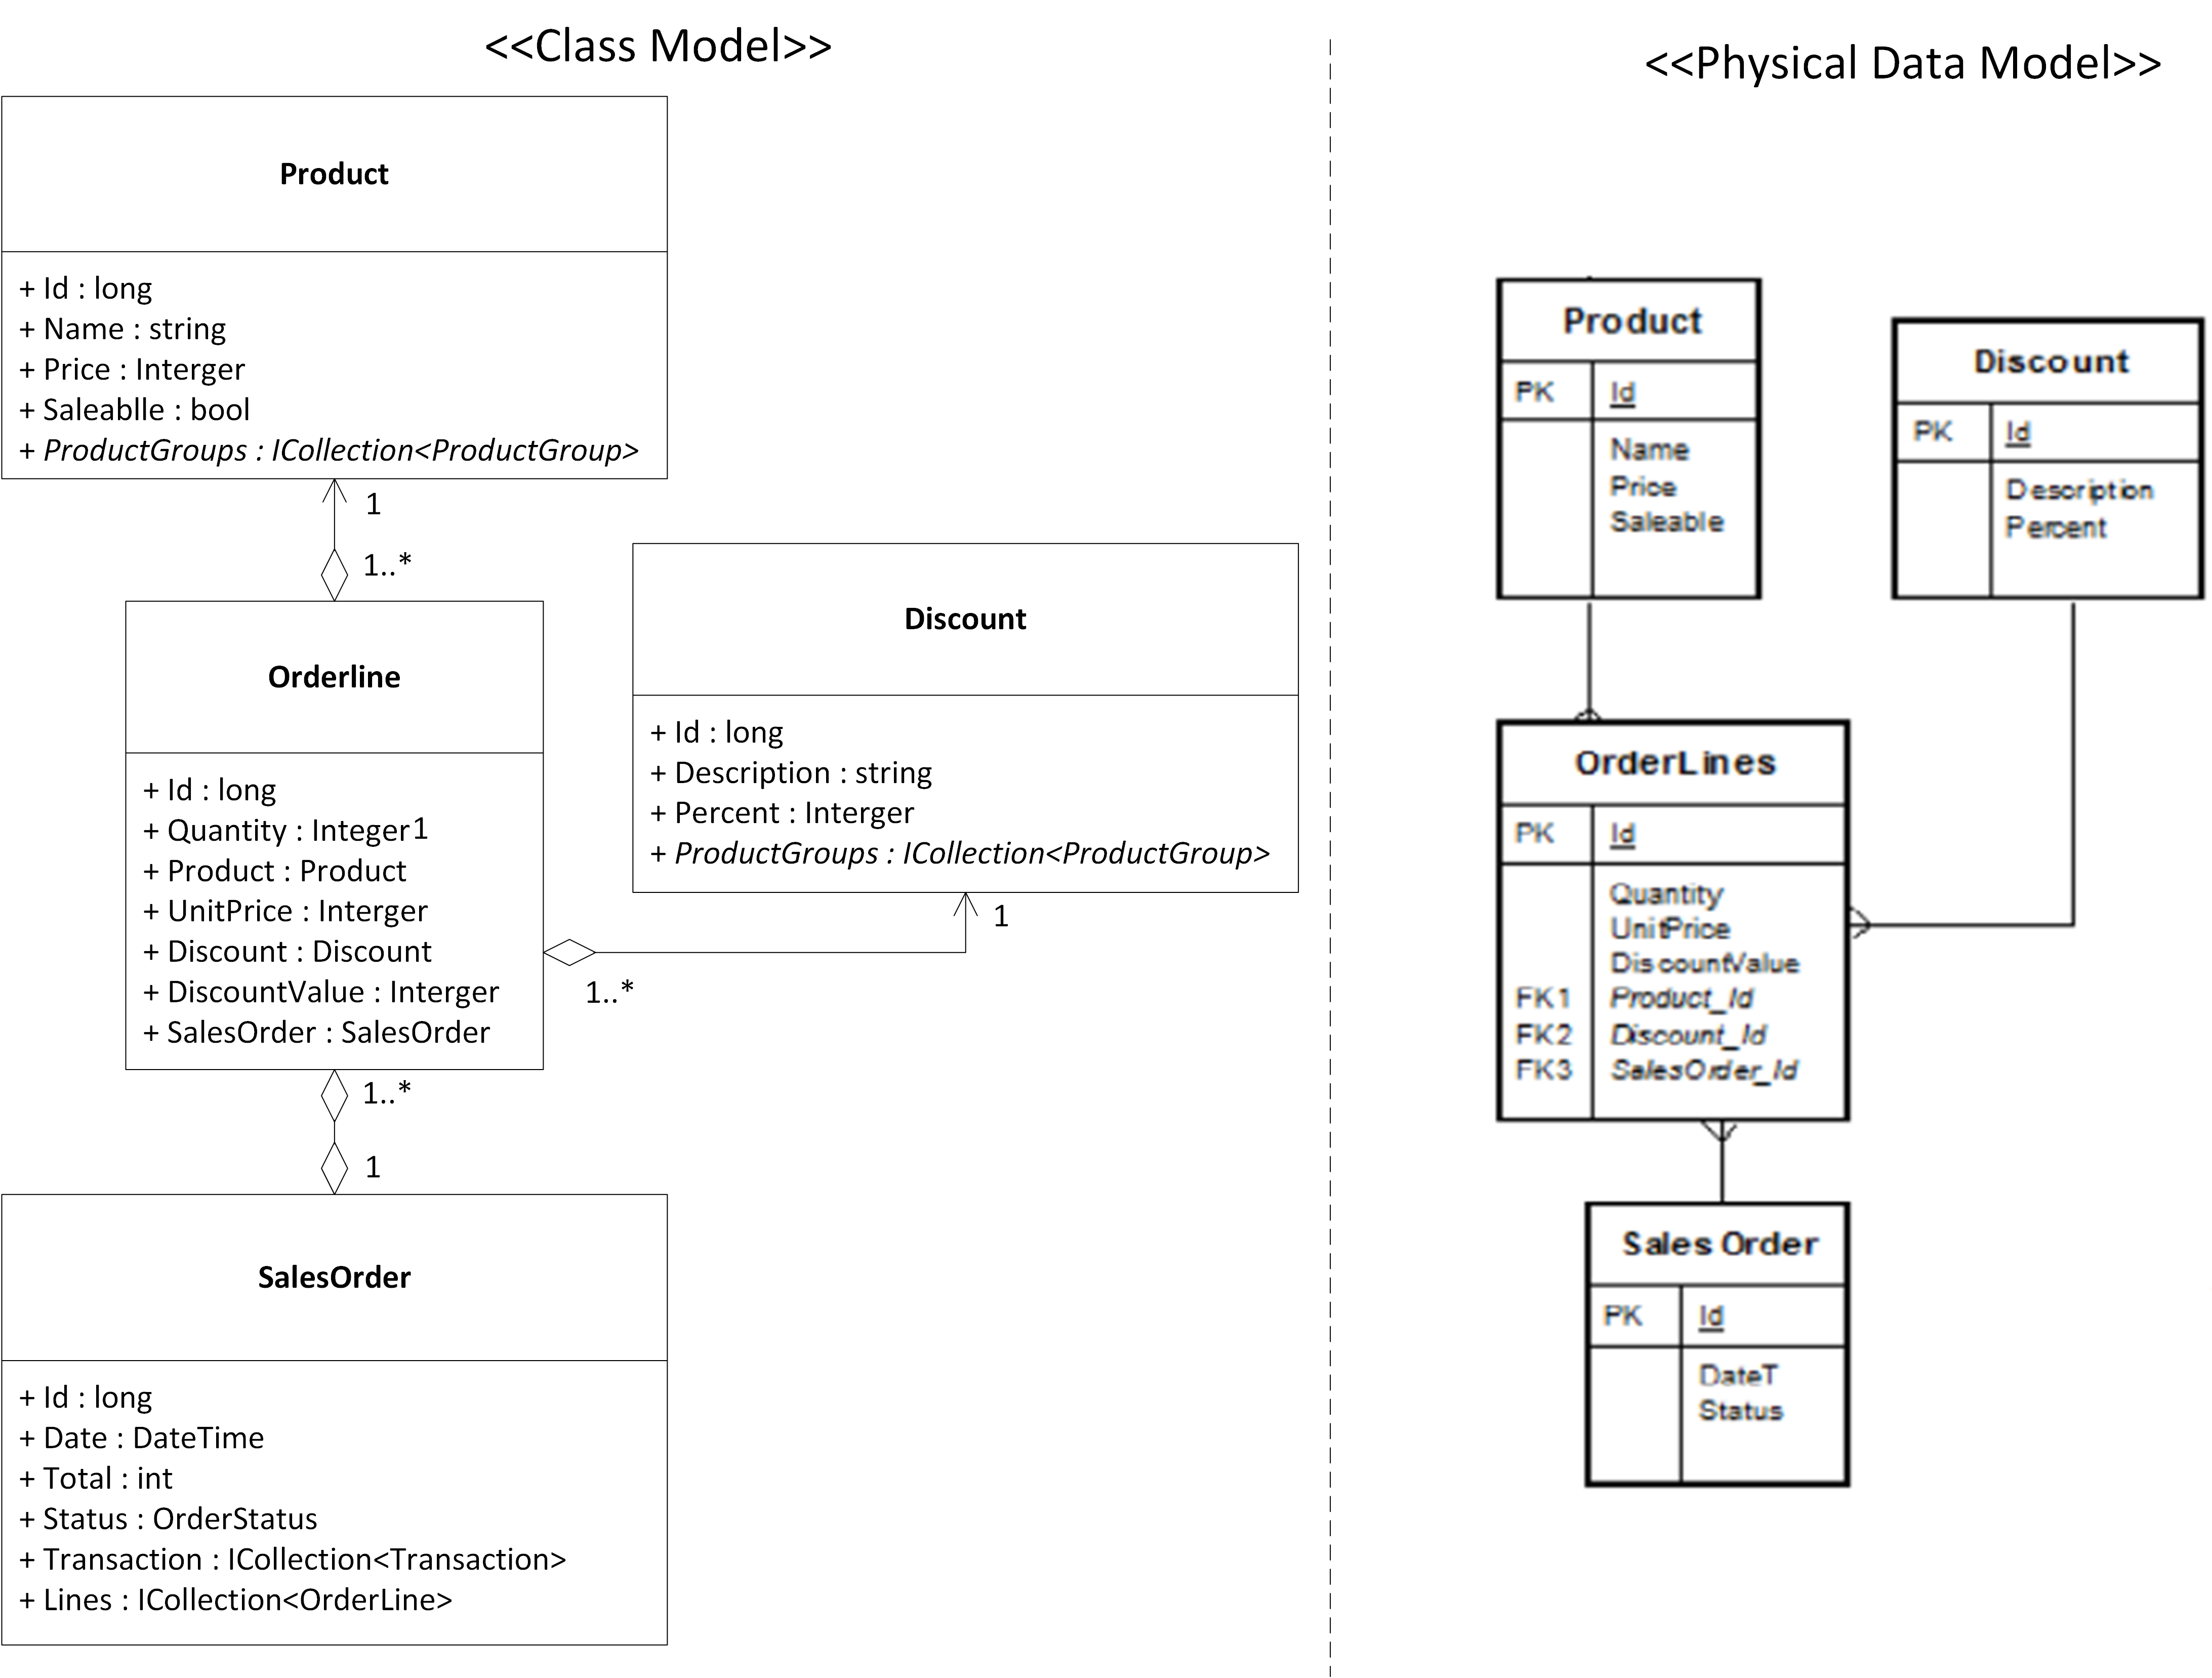
\includegraphics[width=1\textwidth]{N+1/DataView/mapping/Mapping2}
    \caption{Kobling af Orderline}
    \label{fig:Mapping_Orderline}
\end{figure}

OrderLine er sat op så det skal fremstå som køb af en vare. Da Discounts kan anvendes flere gange og der selvfølgeligt kan blive købt mere af det samme Product, skal det være muligt for Discount og Product at være indeholdt i flere OrderLines, derfor er der lavet et one-to-many forhold mellem OrderLine og Product/Disccount, da det er løst med en fremmednøgle i den fysiske database har klasse modelen bare fået en attribut med typen Product og Discount. 
\newline\newline
SalesOrder indholder alle de OrdeLines der er lavet til et køb, derfor er de sat op som en one-to-many tabel, så OrderLine har en fremmednøgle til SalesOrder og SalesOrder har en ICollection af OrderLines så de direkte kan tilgåes ud fra den. 

\subsubsection{ProductGroup}
På figur \ref{fig:Mapping_ProductGroup} ses kobling af Product, Discount og ProductGroup
\begin{figure}[H]
    \centering
    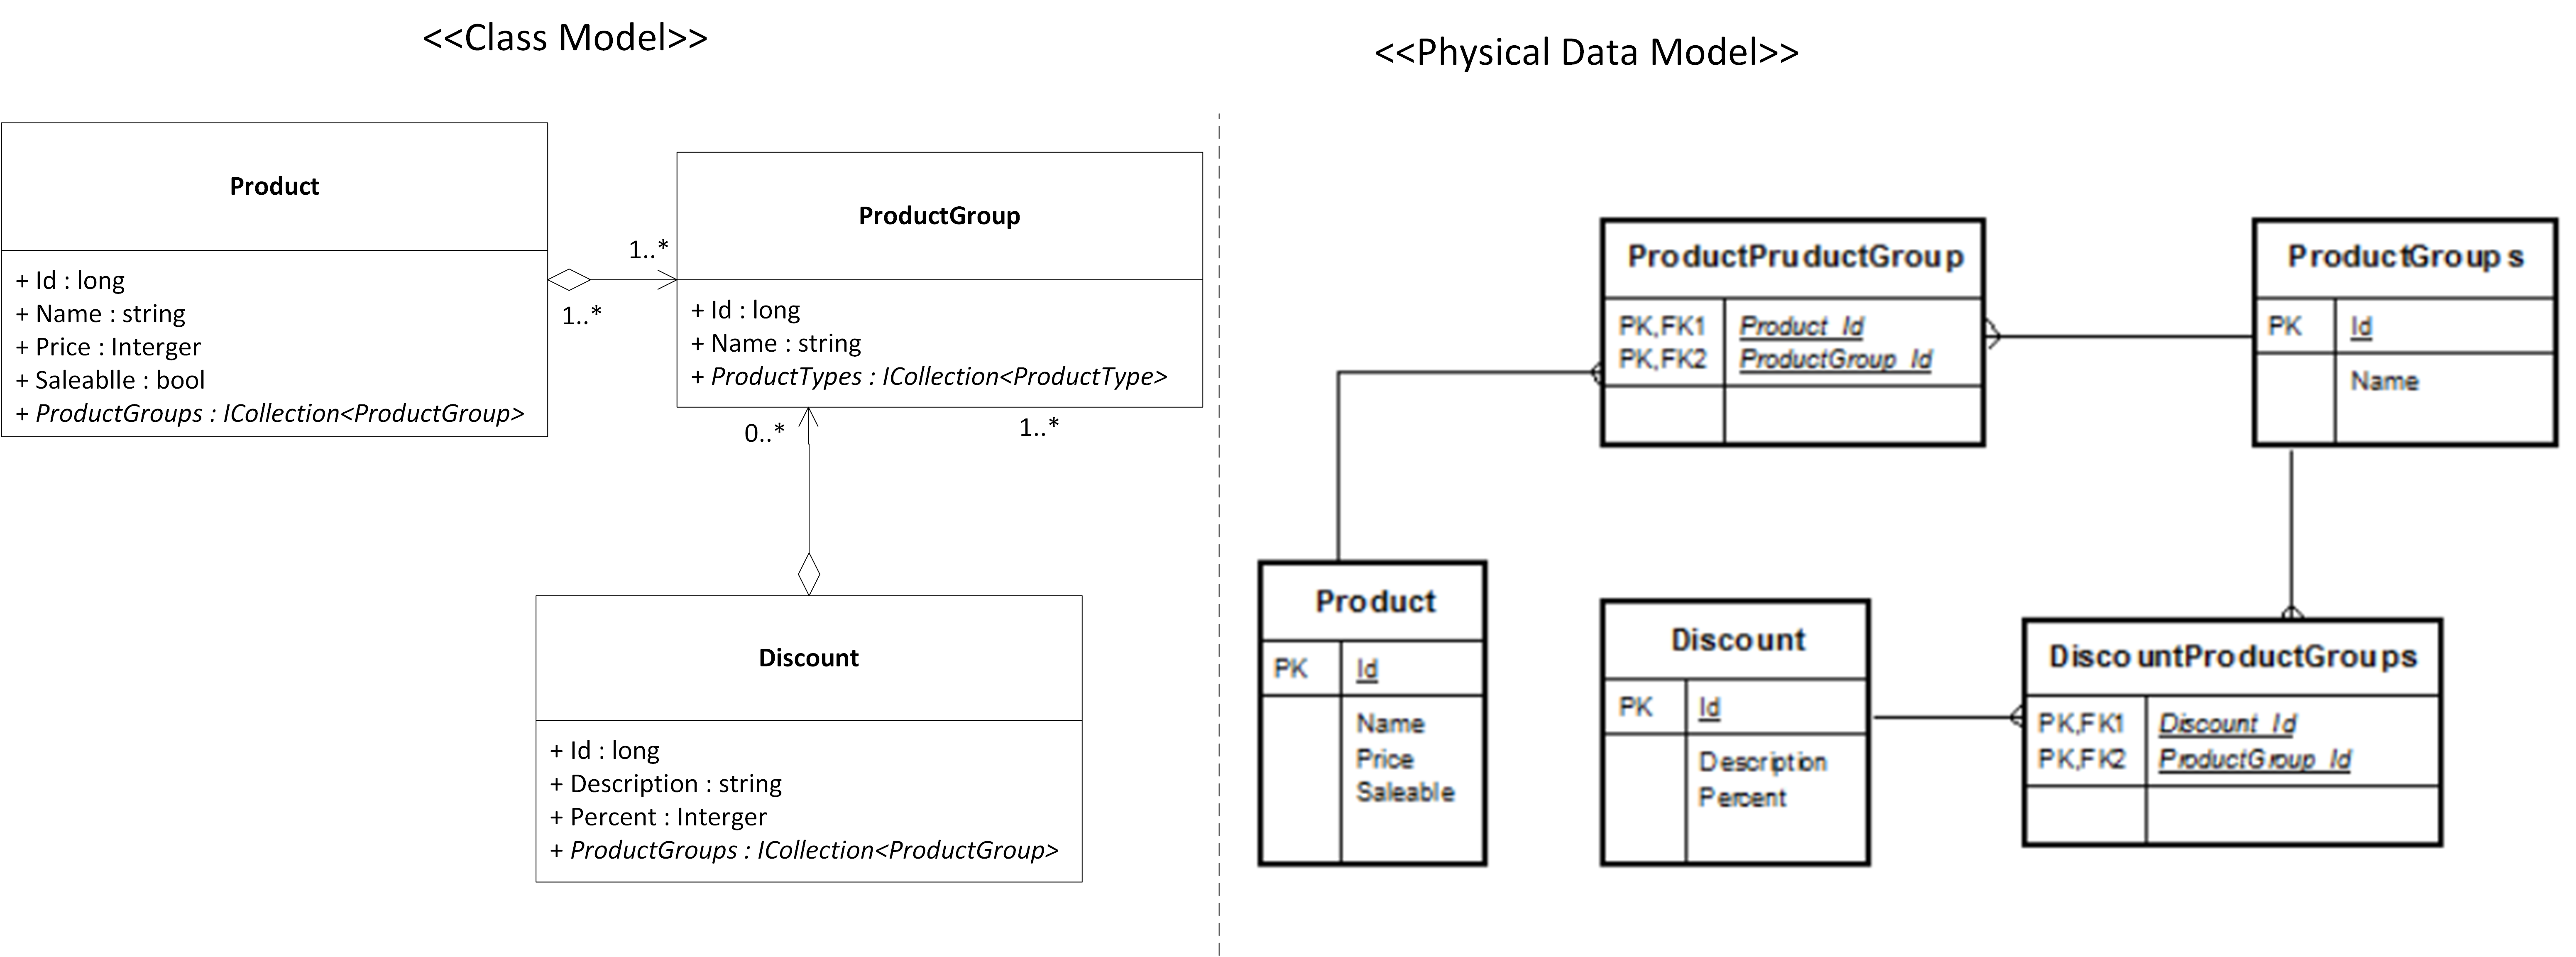
\includegraphics[width=1\textwidth]{N+1/DataView/mapping/Mapping3}
    \caption{Kobling af ProductGroup}
    \label{fig:Mapping_ProductGroup}
\end{figure}

På den fysiske data model kan det ses at Product og Discount har et many-to-many forhold med ProductGroup, da der både kan være flere Producter i en Productgrouppe, men et Product kan også være indeholdt i flere ProductGrouper og det samme gælder på Discount. Dette er løst i klassemodellen ved at give en ICollection af ProductGroups til Discount og Product. 

\subsection{ProductType og ProductTap}

På figur \ref{fig:Mapping_ProductTap_Type} ses kobling af ProductTap, ProductType og ProductGroup

\begin{figure}[H]
    \centering
    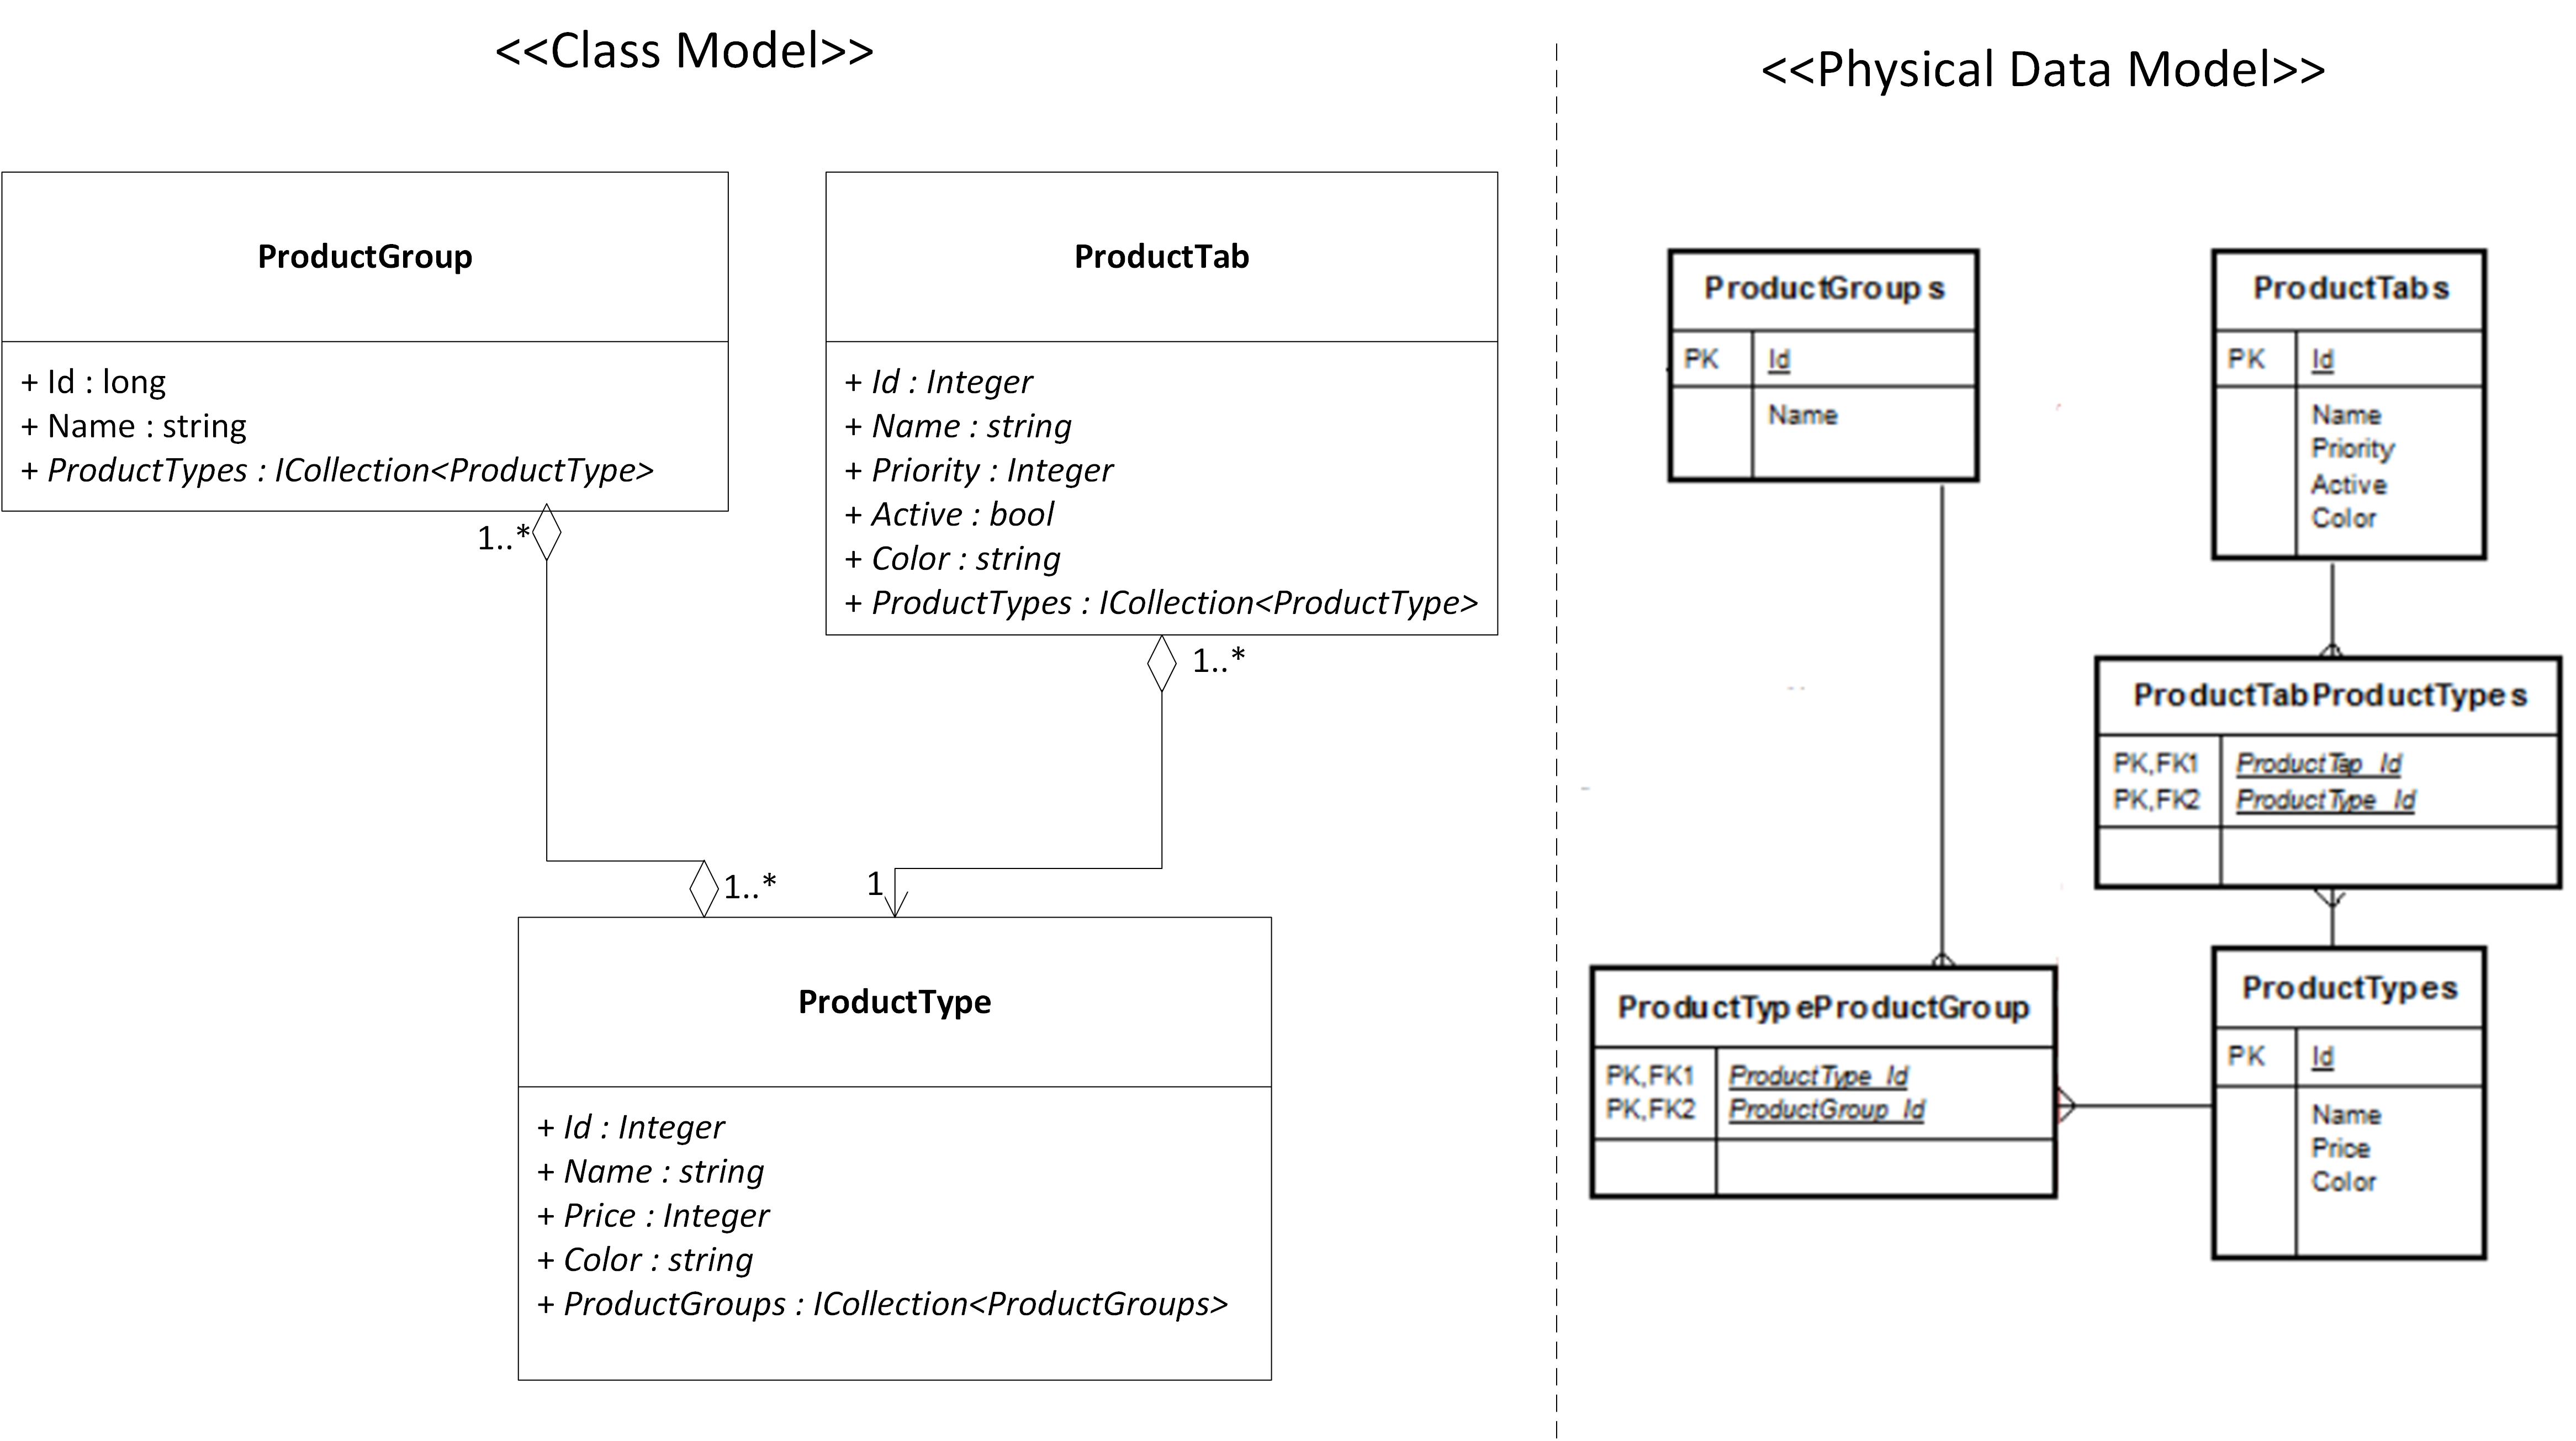
\includegraphics[width=1\textwidth]{N+1/DataView/mapping/Mapping4}
    \caption{Kobling af ProductTap og ProductType}
    \label{fig:Mapping_ProductTap_Type}
\end{figure}

ProductGroup og productType minder meget om hinanden, men ProductGroup kan fungere som undergrupper til ProductType, hvor det skal være muligt at være flere productGrouper under en ProductType, men en ProductGroupe skal også kunne være indeholdt i flere ProductTypes derfor giver det en many-to-many tabel.
\newline
\newline
På GUI'en knapper øverst til højre der har deres information fra ProductTaps i database, ProductTap har et many-to-many forhold med ProductTypes, som er løst i klassemodellen ved at have en ICollection af den anden. 


\subsection{Dataflows}
I følgende afsnit beskrives data flow fra én handling til den næste, ud fra nogle udvalgte use cases, så der kan kommer et indblik på hvornår der bliver hentet, gemt og oprettet data. Her er data flow beskrevet med aktivitetsdiagrammer, hvor det data der går gennem diagrammet er beskrevet med objektnoder. Handlinger er firkanterne med runde hjørner og objektnoderne er firkanterne med skarpe hjørner.   

\subsubsection{UC1 - Kontant salg}
Et kontant salg skal både vise alle de produkter der kan købes, men også gemme salget og transaktionen efter købet er afsluttet. Dette er illustreret på \ref{fig:AD_UC1}

\begin{figure}[H]
    \centering
    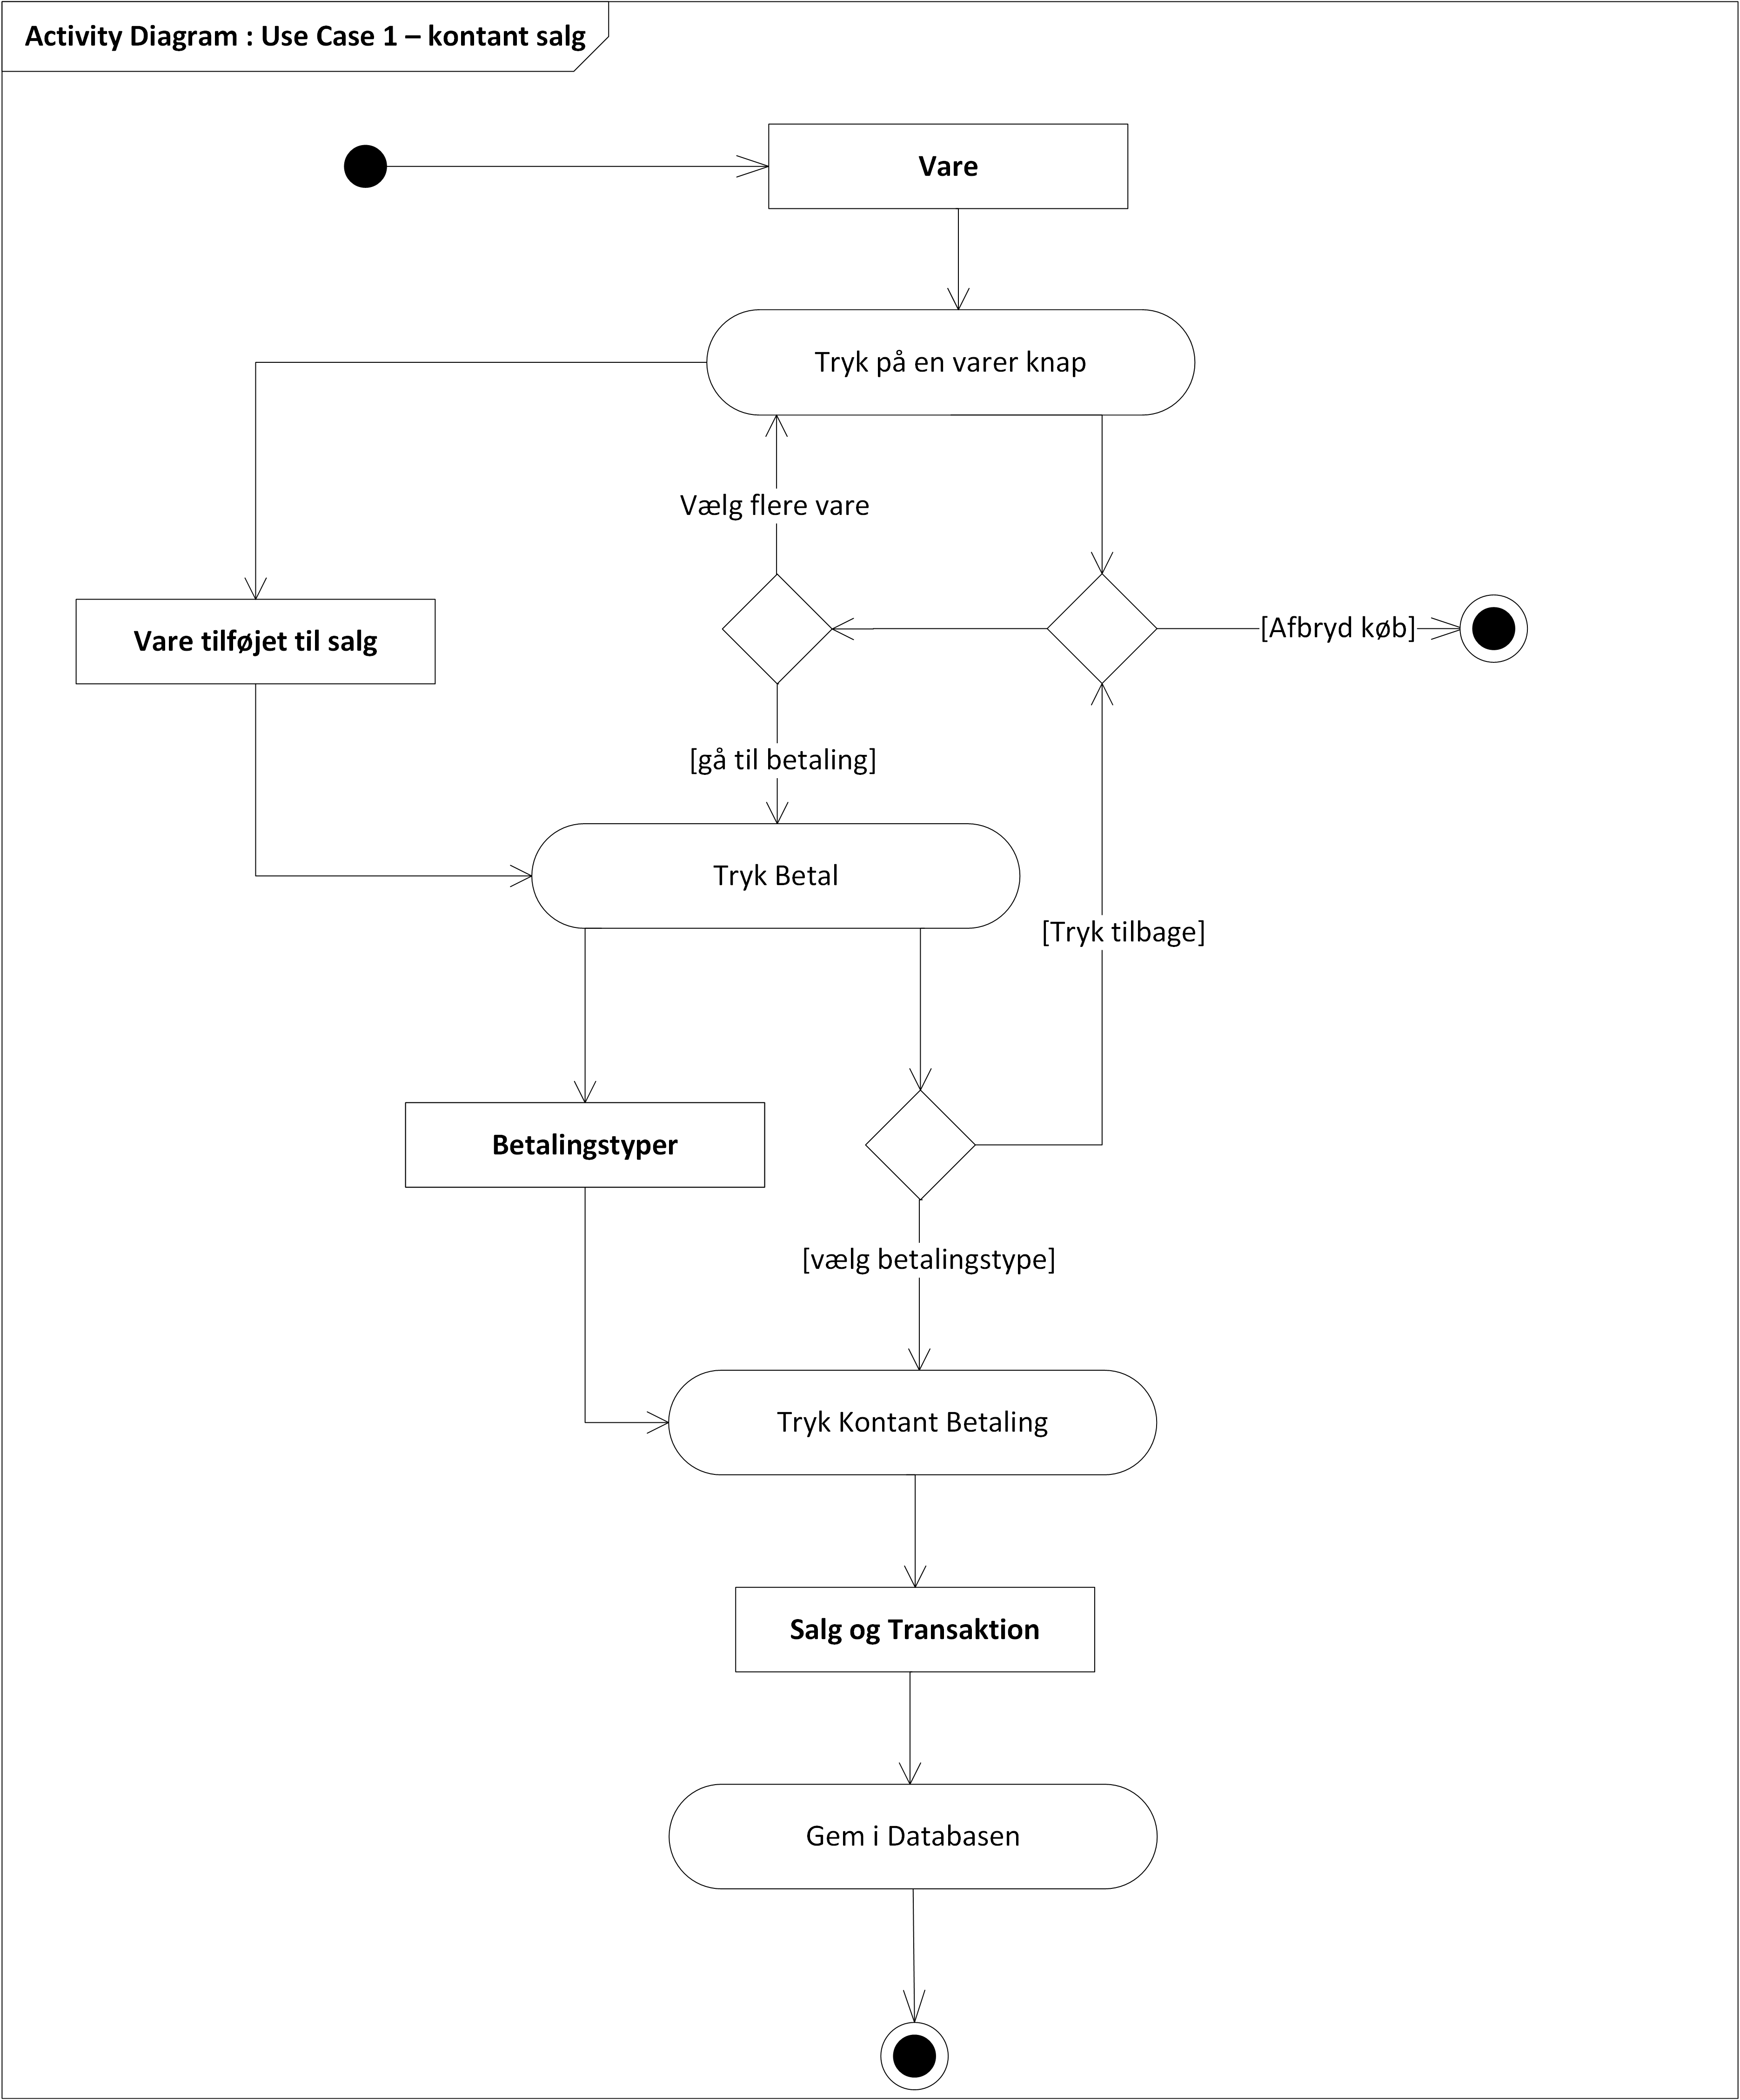
\includegraphics[width=0.8\textwidth]{N+1/DataView/DataFlow/UC1}
    \caption{Aktivitetsdiagram - Kontant salg}
    \label{fig:AD_UC1}
\end{figure}    

Varerne, som hedder Product i databasen, bliver hentet ud så de alle kan ses på GUI'en. Derefter kan man trykke på den vare man ønsker. De valgte varer bliver løbende tilføjet til salget, som i systemet er klassen \texttt{SaleOrder} der kan ses under Model pakken \ref{fig:Models_CLASS}. Når alle de ønskede varer er valgt bliver alle betalingsmuligheder vist og når kontant betaling er trykket, bliver salget og transaktionen gemt i databasen. 

\subsubsection{UC9 - Tilføj varer til kasseapparat}
For at tilføje varer, skal det være muligt at kunne se de allerede eksisterende varer og derefter gemme den vare man ønsker i databasen. Dette er illustreret på \ref{fig:AD_UC9}

\begin{figure}[H]
    \centering
    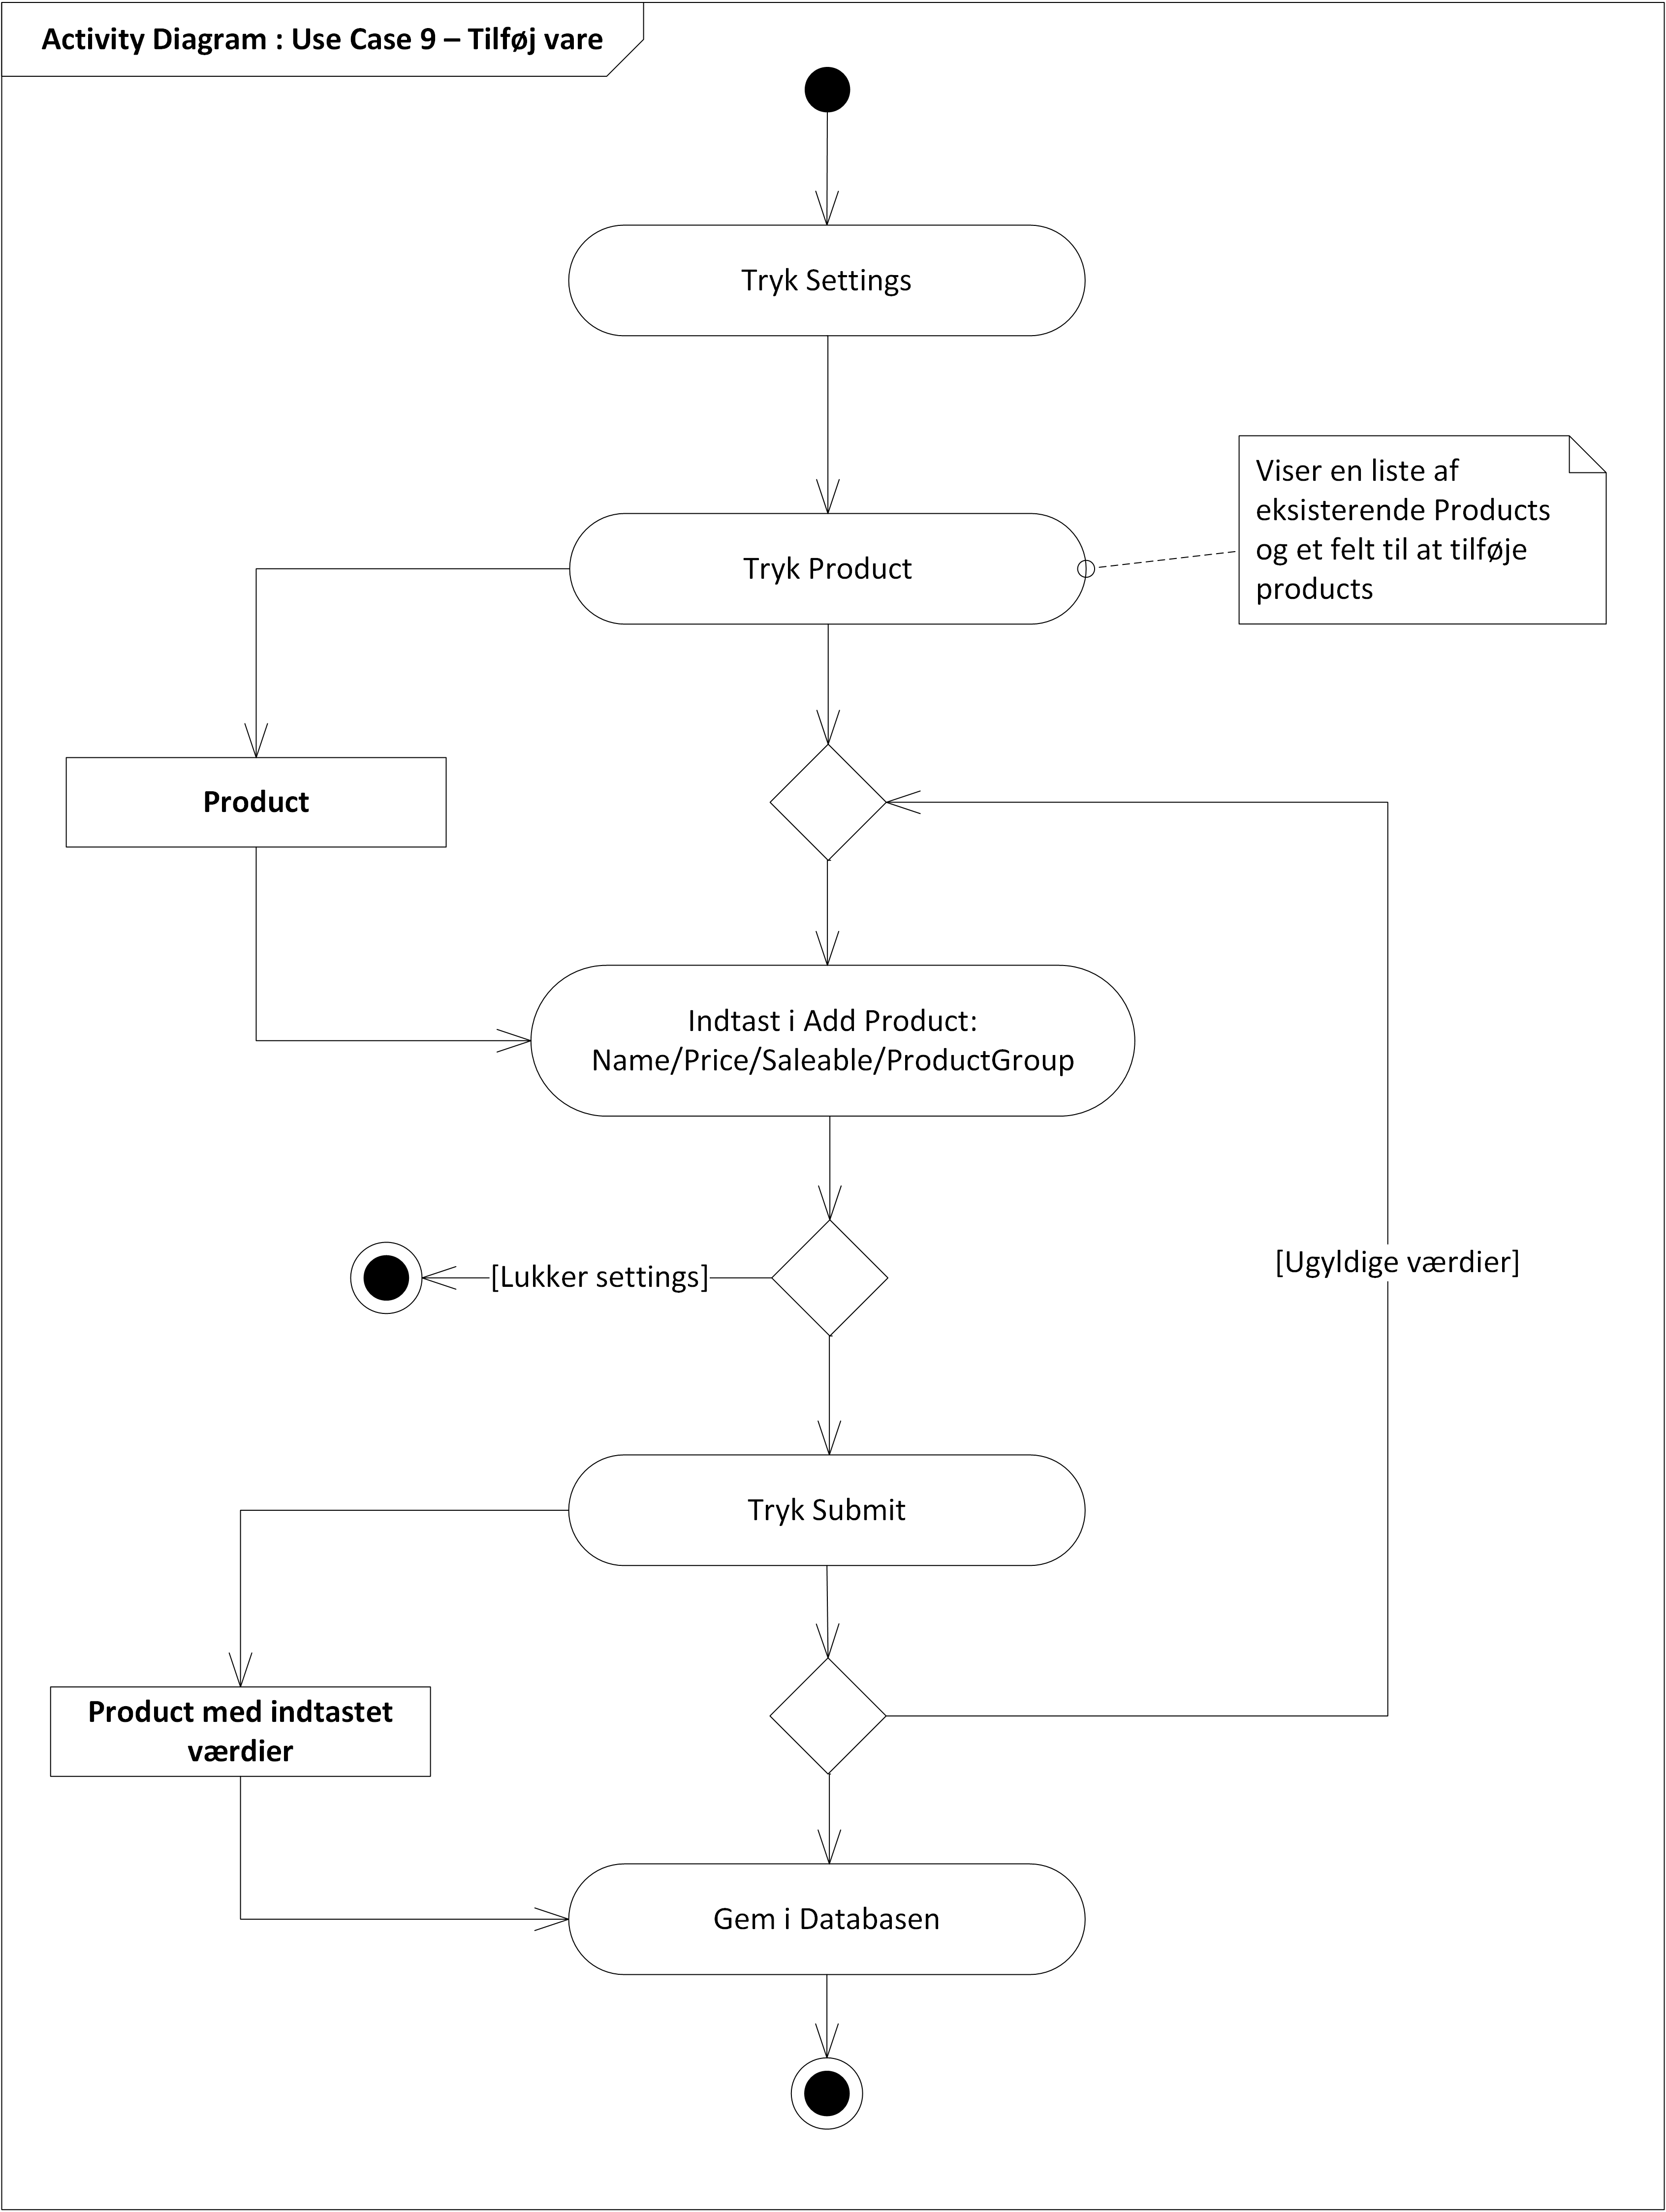
\includegraphics[width=0.8\textwidth]{N+1/DataView/DataFlow/UC9}
    \caption{Aktivitetsdiagram - Tilføj varer til kasseapparat}
    \label{fig:AD_UC9}
\end{figure}    

Varer er gemt som Products, de bliver hentet ud så det er muligt at se hvilke varer der allerede eksisterer i systemet. I feltet hvor man kan tilføje vare udfylder man alle dens værdier, hvis værdierne er gyldige bliver de gemt i databasen. 

\subsection{UC12 - Vis statistik over salg}
Det skal være muligt at se de salg der har været foretaget tidligere i systemet. Alle salg bliver løbende gemt i databasen, hvor de derefter kan ses under statestic i Web Api'et. Dette er illustreret på \ref{fig:AD_UC12}

\begin{figure}[H]
    \centering
    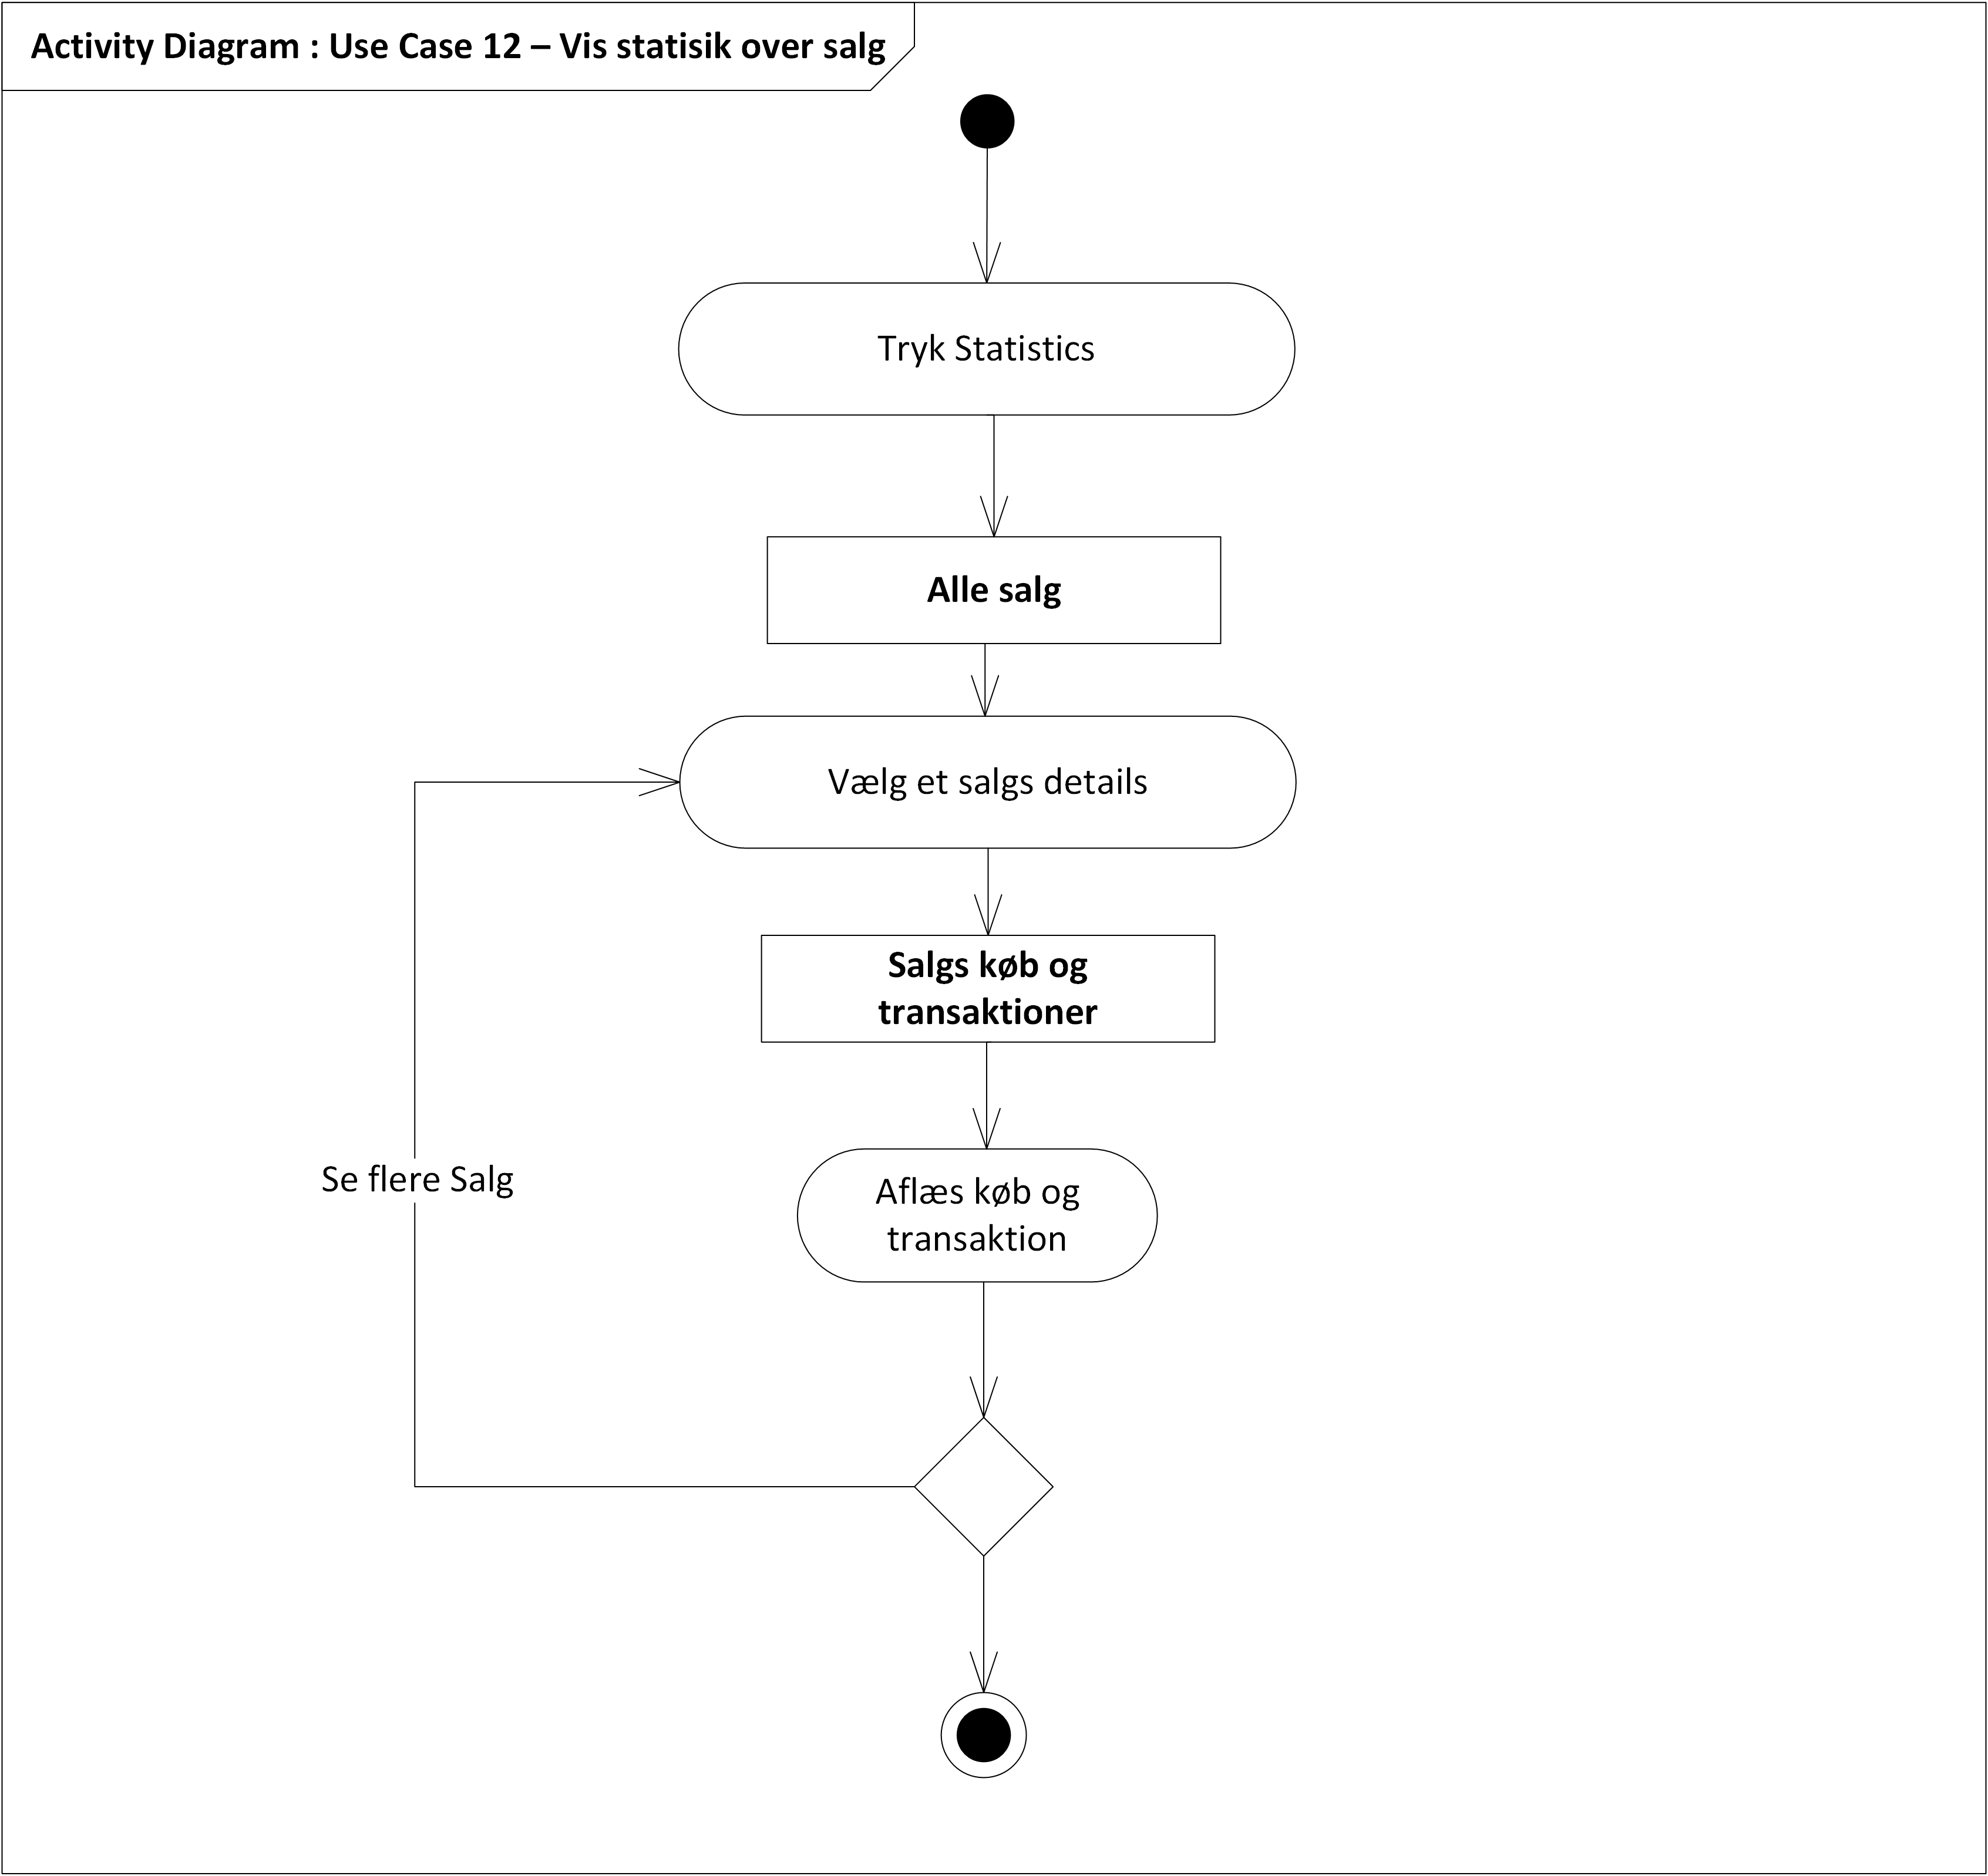
\includegraphics[width=0.8\textwidth]{N+1/DataView/DataFlow/UC12}
    \caption{Aktivitetsdiagram - Vis statistik over salg}
    \label{fig:AD_UC12}
\end{figure} 

Statistic viser en side over alle salg de salg der har været. I databasen hedder disse salg, \texttt{SalesOrder}. Her kan man gå ind under alle salg og se detaljer om de varer der er købt og hvordan transaktionerne forløb. 



%Generelle Designbeslutninger
\section{Generelle Designbeslutninger}

\subsection{Databasestrukturen}
Den centrale database, der kan placeres lokalt på en computer eller på en central server, er designet ud fra at kunne tilføje nye produkter, produkttyper og produktfaner samt udnytte at produktgrupper er en samling af produkter, så en produktgruppe både kan bestemme hvilken type produkterne hører til og hvilken discount de skal kunne bruges sammen med.

\subsection{Programmeringsprog}
C\# blev valgt på baggrund af Entity Frameworket til at forbinde til databasen og WPF til selve GUI'en. Desuden er 4 semesters undervisning i Database, Softwaretest og GUI centreret omkring C\#. Til webapi blev der brugt ASP.NET, da denne også kan benytte sig af Entity Frameworket.

\subsection{Testing}
NUnit, NSubstitute, dotCover og FxCop blev anvendt til dette job eftersom vi allerede brugte C\# som programmeringssprog, og disse tests er lette at automatisere.

\subsection{Dokumentation}
LaTeX blev valgt grundet dets egenskab til at flere kan let arbejde på samme dokument, samt revisionering er utrolig let. Doxygen blev brugt til at lave dokumentation af selve softwaren.

\subsection{Automatisering}
TeamCity blev valgt til automatisere unit og integrationstests. Dette blev koblet sammen med Github til at trikke hver gang et Pull Request blev lavet se mere under Change Management.
En kombination af Docker, Doxygen, TexLive og bashscript, sørgede for at bygge dokumentationen hver gang der kom en update til masteren. Dette blev published til en webserver, derved er der altid adgang til nyeste dokumentation.


\subsection{Implementeringsværktøjer}
\begin{description}
  \item[Microsoft Visual Studio 2015] \hfill \\
  Er brugt til at udvikle core biblioteket, samt websiden og selve gui\'en
  \item[ReSharper from JetBrains] \hfill \\
  Til at hjælp med kode analyse, find mulige runtime fejl, og hjælpe med sanity tjek af variabler.
  \item[NUnit] \hfill \\
  Bruges til Unit og Integrationstest. De blev valgt på baggrund af deres lette framework op mod C\#.
  \item[Github] \hfill \\
  Revisionsprogram der er brugt for at sikre kodereview via Pull-Requests. Når en person har lavet en ønsket ændring, lægges denne op på github, hvor en anden person kigger ændringen igennem inden den merges ind med vores master \citeauthor{gh:pullrequests}. Github er også sat op til at samarbejde med TeamCity (se nedenunder)
  \item[TeamCity] \hfill \\
  TeamCity er blev brugt som build server og test server. Vi har sat vores egen TeamCity server op, som kommunikerede med Github for at sikre at Pull-Requests kunne bygge.
  \item[DDS-Lite] \hfill \\
  Er brugt til at designe database layoutet.
\end{description}

\subsection{Dokumentationsværktøjer}
\begin{description}
  \item[Texmaker] \hfill \\
  Vores rapport og dokumentation er hovedsageligt skrevet i Latex, og vi har brugt Texmaker til dette.
  \item[Visio] \hfill \\
  Brugt til diverse diagrammer.
  \item[Dockerized pdflatex] \hfill \\
  Brugt til automatisk bygning af dokumentation og rapport. Dette er et selvbygget program der henter den nyeste version fra Github, kompilerere rapporten og dokumentationen, og udgiver den til en webserver.
  \item[Dockerized Doxygen] \hfill \\
  Brugt til automatisk bygning af dokumentation af C\# koden. Er også lavet til at hente den nyeste master, kompilere dokumentationen for CashRegister og CashRegister.WebApi, og udgive den på en webserver.
\end{description}

\subsection{Change Management}
Der blev brugt en Change Management metode for at sikre, at der ikke kom utilsigtigede ændringer ind. Processen er groft tegnet i \ref{fig:ChangeManagement_SEQ}. Flowet kan bedst beskrives som følgende
\begin{enumerate}[label=\arabic{enumi}.,ref=\arabic{enumi}]
  \item \label{editorstart} En Editor laver nogle ændringer og laver et Pull Request
  \item Github tager fat i TeamCity serveren, og informerer at der er kommet et nyt Pull Request
  \item TeamCity serveren bygger og kører unit, integration og fxcop tests. Dette meldes tilbage til Github, samt kan man fra Github gå direkte til build processen på TeamCity serveren.
  \item Hvis der er fejl lukkes Pull Requesten af Reviewer og Editor begynder fra \ref{editorstart}.
  \item Hvis alle tests går godt kigger Reviewer ændringerne igennem for at gribe fejl der ikke umiddelbart kan testes for. Dette kunne være unødvendige filer, giberish der er glemt at blive rettet, ændringer der designmæssigt er forkerte mm.
  \item Hvis ovenstående bliver godkendt af Reviewer, merger Reviewer Pull Requesten og denne lukkes.
  \item Hvis ændringer ikke kan godkendes begynder Reviewer fra \ref{editorstart}.
\end{enumerate}

Et sekundært afkast er at dette hjælper med at mindske, at merge konflikter kommer ind i masteren. Et eksempel kunne være følgende stykke kode.
\begin{lstlisting}
// Vis vores Item paa skaermen
public void ShowItem(Item item, string prefix)
{
    Console.Write(item);
}
\end{lstlisting}
Det kan tydeligt ses at variablen prefix ikke bliver brugt. Person A og B begynder nu begge at ændre på denne fil. Person A fjerner prefix variablen da denne jo ikke er i brug.
\begin{lstlisting}
// Vis vores Item paa skaermen
public void ShowItem(Item item)
{
    Console.Write(item);
}
\end{lstlisting}
Person B derimod har opdaget at han har glemt at bruge prefix, og retter sin fejl.
\begin{lstlisting}
// Vis vores Item paa skaermen
public void ShowItem(Item item, string prefix)
{
    Console.Write(prefix + " " + item);
}
\end{lstlisting}
Begge disse ændringer ville let kunne merges rent teknisk, da ændringerne er langt nok fra hinanden.
\begin{lstlisting}
// Vis vores Item paa skaermen
public void ShowItem(Item item)
{
    Console.Write(prefix + " " + item);
}
\end{lstlisting}
Dog kan filen nu ikke kompileres længere! Dette løses med ovenstående Change Management, da nummer 2 Pull Request ville blive afvist af TeamCity. 
\sysml{0.9}{SEQ}{ChangeManagement}{Change Management}
